\documentclass[a4paper, 12pt]{book}
%\documentclass[a4paper, 12pt, draft]{book}  Nalogo preverite tudi z opcijo draft, ki vam bo pokazala, katere vrstice so predolge!



\usepackage[utf8x]{inputenc}   % omogoča uporabo slovenskih črk kodiranih v formatu UTF-8
\usepackage[slovene,english]{babel}    % naloži, med drugim, slovenske delilne vzorce
\usepackage[pdftex]{graphicx}  % omogoča vlaganje slik različnih formatov
\usepackage{fancyhdr}          % poskrbi, na primer, za glave strani
\usepackage{amssymb}           % dodatni simboli
\usepackage{amsmath}           % eqref, npr.
%\usepackage{hyperxmp}
\usepackage[hyphens]{url}  % dodal Solina
\usepackage{comment}       % dodal Solina

\usepackage[pdftex, colorlinks=true,
						citecolor=black, filecolor=black, 
						linkcolor=black, urlcolor=black,
						pagebackref=false, 
						pdfproducer={LaTeX}, pdfcreator={LaTeX}, hidelinks]{hyperref}

\usepackage{color}       % dodal Solina
\usepackage{soul}       % dodal Solina

\usepackage[section]{placeins}

\usepackage{listings}
\lstset{basicstyle=\footnotesize\ttfamily}
\renewcommand{\lstlistingname}{Izsek izvorne kode}% Listing -> Algorithm
\renewcommand{\lstlistlistingname}{Seznam izsekov izvorne kode}% List of Listings -> List of Algorithms

%%%%%%%%%%%%%%%%%%%%%%%%%%%%%%%%%%%%%%%%
%	DIPLOMA INFO
%%%%%%%%%%%%%%%%%%%%%%%%%%%%%%%%%%%%%%%%
\newcommand{\ttitle}{Zasnova in razvoj platforme za spremljanje metrik HTML5 spletnih aplikacij}
\newcommand{\ttitleEn}{Design and implementation of platform for monitoring metrics of HTML5 web applications}
\newcommand{\tsubject}{\ttitle}
\newcommand{\tsubjectEn}{\ttitleEn}
\newcommand{\tauthor}{Miha Jamšek}
\newcommand{\tkeywords}{metrike, html, html5, splet, spletne aplikacije, spa, platforma, rum, spremljanje, čas nalaganja}
\newcommand{\tkeywordsEn}{metrics, html, html5, web, web applications, spa, platform, rum, monitoring, load time}


%%%%%%%%%%%%%%%%%%%%%%%%%%%%%%%%%%%%%%%%
%	HYPERREF SETUP
%%%%%%%%%%%%%%%%%%%%%%%%%%%%%%%%%%%%%%%%
\hypersetup{pdftitle={\ttitle}}
\hypersetup{pdfsubject=\ttitleEn}
\hypersetup{pdfauthor={\tauthor, mj6243@student.uni-lj.si}}
\hypersetup{pdfkeywords=\tkeywordsEn}


 


%%%%%%%%%%%%%%%%%%%%%%%%%%%%%%%%%%%%%%%%
% postavitev strani
%%%%%%%%%%%%%%%%%%%%%%%%%%%%%%%%%%%%%%%%  

\addtolength{\marginparwidth}{-20pt} % robovi za tisk
\addtolength{\oddsidemargin}{40pt}
\addtolength{\evensidemargin}{-40pt}

\renewcommand{\baselinestretch}{1.3} % ustrezen razmik med vrsticami
\setlength{\headheight}{15pt}        % potreben prostor na vrhu
\renewcommand{\chaptermark}[1]%
{\markboth{\MakeUppercase{\thechapter.\ #1}}{}} \renewcommand{\sectionmark}[1]%
{\markright{\MakeUppercase{\thesection.\ #1}}} \renewcommand{\headrulewidth}{0.5pt} \renewcommand{\footrulewidth}{0pt}
\fancyhf{}
\fancyhead[LE,RO]{\sl \thepage} 
%\fancyhead[LO]{\sl \rightmark} \fancyhead[RE]{\sl \leftmark}
\fancyhead[RE]{\sc \tauthor}              % dodal Solina
\fancyhead[LO]{\sc Diplomska naloga}     % dodal Solina


\newcommand{\BibTeX}{{\sc Bib}\TeX}

%%%%%%%%%%%%%%%%%%%%%%%%%%%%%%%%%%%%%%%%
% naslovi
%%%%%%%%%%%%%%%%%%%%%%%%%%%%%%%%%%%%%%%%  


\newcommand{\autfont}{\Large}
\newcommand{\titfont}{\LARGE\bf}
\newcommand{\clearemptydoublepage}{\newpage{\pagestyle{empty}\cleardoublepage}}
\setcounter{tocdepth}{1}	      % globina kazala

%%%%%%%%%%%%%%%%%%%%%%%%%%%%%%%%%%%%%%%%
% konstrukti
%%%%%%%%%%%%%%%%%%%%%%%%%%%%%%%%%%%%%%%%  
\newtheorem{izrek}{Izrek}[chapter]
\newtheorem{trditev}{Trditev}[izrek]
\newenvironment{dokaz}{\emph{Dokaz.}\ }{\hspace{\fill}{$\Box$}}

%%%%%%%%%%%%%%%%%%%%%%%%%%%%%%%%%%%%%%%%%%%%%%%%%%%%%%%%%%%%%%%%%%%%%%%%%%%%%%%
%% PDF-A
%%%%%%%%%%%%%%%%%%%%%%%%%%%%%%%%%%%%%%%%%%%%%%%%%%%%%%%%%%%%%%%%%%%%%%%%%%%%%%%


%%%%%%%%%%%%%%%%%%%%%%%%%%%%%%%%%%%%%%%% 
% define medatata
%%%%%%%%%%%%%%%%%%%%%%%%%%%%%%%%%%%%%%%% 
\def\Title{\ttitle}
\def\Author{\tauthor, mj6243@student.uni-lj.si}
\def\Subject{\ttitleEn}
\def\Keywords{\tkeywordsEn}

%%%%%%%%%%%%%%%%%%%%%%%%%%%%%%%%%%%%%%%% 
% \convertDate converts D:20080419103507+02'00' to 2008-04-19T10:35:07+02:00
%%%%%%%%%%%%%%%%%%%%%%%%%%%%%%%%%%%%%%%% 
\def\convertDate{%
    \getYear
}

{\catcode`\D=12
 \gdef\getYear D:#1#2#3#4{\edef\xYear{#1#2#3#4}\getMonth}
}
\def\getMonth#1#2{\edef\xMonth{#1#2}\getDay}
\def\getDay#1#2{\edef\xDay{#1#2}\getHour}
\def\getHour#1#2{\edef\xHour{#1#2}\getMin}
\def\getMin#1#2{\edef\xMin{#1#2}\getSec}
\def\getSec#1#2{\edef\xSec{#1#2}\getTZh}
\def\getTZh +#1#2{\edef\xTZh{#1#2}\getTZm}
\def\getTZm '#1#2'{%
    \edef\xTZm{#1#2}%
    \edef\convDate{\xYear-\xMonth-\xDay T\xHour:\xMin:\xSec+\xTZh:\xTZm}%
}

\expandafter\convertDate\pdfcreationdate 

%%%%%%%%%%%%%%%%%%%%%%%%%%%%%%%%%%%%%%%%
% get pdftex version string
%%%%%%%%%%%%%%%%%%%%%%%%%%%%%%%%%%%%%%%% 
\newcount\countA
\countA=\pdftexversion
\advance \countA by -100
\def\pdftexVersionStr{pdfTeX-1.\the\countA.\pdftexrevision}


%%%%%%%%%%%%%%%%%%%%%%%%%%%%%%%%%%%%%%%%
% XMP data
%%%%%%%%%%%%%%%%%%%%%%%%%%%%%%%%%%%%%%%%  
\usepackage{xmpincl}
\includexmp{pdfa-1b}

%%%%%%%%%%%%%%%%%%%%%%%%%%%%%%%%%%%%%%%%
% pdfInfo
%%%%%%%%%%%%%%%%%%%%%%%%%%%%%%%%%%%%%%%%  
\pdfinfo{%
    /Title    (\ttitle)
    /Author   (\tauthor, mj6243@student.uni-lj.si)
    /Subject  (\ttitleEn)
    /Keywords (\tkeywordsEn)
    /ModDate  (\pdfcreationdate)
    /Trapped  /False
}


%%%%%%%%%%%%%%%%%%%%%%%%%%%%%%%%%%%%%%%%%%%%%%%%%%%%%%%%%%%%%%%%%%%%%%%%%%%%%%%
%%%%%%%%%%%%%%%%%%%%%%%%%%%%%%%%%%%%%%%%%%%%%%%%%%%%%%%%%%%%%%%%%%%%%%%%%%%%%%%

\begin{document}
\selectlanguage{slovene}
\frontmatter
\setcounter{page}{1} %
\renewcommand{\thepage}{}       % preprecimo težave s številkami strani v kazalu
\newcommand{\sn}[1]{"`#1"'}                    % dodal Solina (slovenski narekovaji)

%%%%%%%%%%%%%%%%%%%%%%%%%%%%%%%%%%%%%%%%
%naslovnica
 \thispagestyle{empty}%
   \begin{center}
    {\large\sc Univerza v Ljubljani\\%
      Fakulteta za računalništvo in informatiko}%
    \vskip 10em%
    {\autfont \tauthor\par}%
    {\titfont \ttitle \par}%
    {\vskip 3em \textsc{DIPLOMSKO DELO\\[5mm]         % dodal Solina za ostale študijske programe
%    VISOKOŠOLSKI STROKOVNI ŠTUDIJSKI PROGRAM\\ PRVE STOPNJE\\ RAČUNALNIŠTVO IN INFORMATIKA}\par}%
    UNIVERZITETNI  ŠTUDIJSKI PROGRAM\\ PRVE STOPNJE\\ RAČUNALNIŠTVO IN INFORMATIKA}\par}%
%    INTERDISCIPLINARNI UNIVERZITETNI\\ ŠTUDIJSKI PROGRAM PRVE STOPNJE\\ RAČUNALNIŠTVO IN MATEMATIKA}\par}%
%    INTERDISCIPLINARNI UNIVERZITETNI\\ ŠTUDIJSKI PROGRAM PRVE STOPNJE\\ UPRAVNA INFORMATIKA}\par}%
%    INTERDISCIPLINARNI UNIVERZITETNI\\ ŠTUDIJSKI PROGRAM PRVE STOPNJE\\ MULTIMEDIJA}\par}%
    \vfill\null%
    {\large \textsc{Mentor}: prof. dr. Matjaž B. Jurič\par}%
    {\vskip 2em \large Ljubljana, 2019 \par}%
\end{center}
% prazna stran
%\clearemptydoublepage      % dodal Solina (izjava o licencah itd. se izpiše na hrbtni strani naslovnice)

%%%%%%%%%%%%%%%%%%%%%%%%%%%%%%%%%%%%%%%%
%copyright stran
\thispagestyle{empty}
\vspace*{8cm}

\noindent
{\sc Copyright}. 
Rezultati diplomske naloge so intelektualna lastnina avtorja in Fakultete za računalništvo in informatiko Univerze v Ljubljani.
Za objavo in koriščenje rezultatov diplomske naloge je potrebno pisno privoljenje avtorja, Fakultete za računalništvo in informatiko ter mentorja.
Izvorna koda diplomskega dela, njeni rezultati in v ta namen razvita programska oprema je ponujena pod odprtokodno licenco MIT. Podrobnosti licence so dostopne na spletni strani https://opensource.org/licenses/MIT.

\begin{center}
\mbox{}\vfill
\emph{Besedilo je oblikovano z urejevalnikom besedil \LaTeX.}
\end{center}
% prazna stran
\clearemptydoublepage

%%%%%%%%%%%%%%%%%%%%%%%%%%%%%%%%%%%%%%%%
% stran 3 med uvodnimi listi
\thispagestyle{empty}
\vspace*{4cm}

\noindent
Fakulteta za računalništvo in informatiko izdaja naslednjo nalogo:
\medskip
\begin{tabbing}
\hspace{32mm}\= \hspace{6cm} \= \kill




Tematika naloge:
\end{tabbing}
TODO
\vspace{15mm}






\vspace{2cm}

% prazna stran
\clearemptydoublepage

% zahvala
\thispagestyle{empty}\mbox{}\vfill\null\it%
\noindent
TODO
\rm\normalfont

% prazna stran
\clearemptydoublepage

%%%%%%%%%%%%%%%%%%%%%%%%%%%%%%%%%%%%%%%%

% prazna stran
\clearemptydoublepage


%%%%%%%%%%%%%%%%%%%%%%%%%%%%%%%%%%%%%%%%
% kazalo
\pagestyle{empty}
\def\thepage{}% preprecimo tezave s stevilkami strani v kazalu
\tableofcontents{}


% prazna stran
\clearemptydoublepage

%%%%%%%%%%%%%%%%%%%%%%%%%%%%%%%%%%%%%%%%
% seznam kratic

\chapter*{Seznam uporabljenih kratic}  % spremenil Solina, da predolge vrstice ne gredo preko desnega roba

\begin{comment}

\begin{tabular}{l|l|l}
  {\bf kratica} & {\bf angleško} & {\bf slovensko} \\ \hline
  % after \\: \hline or \cline{col1-col2} \cline{col3-col4} ...
  {\bf CA} & classification accuracy & klasifikacijska točnost \\
  {\bf DBMS} & database management system & sistem za upravljanje podatkovnih baz \\
  {\bf SVM} & support vector machine & metoda podpornih vektorjev \\
  \dots & \dots & \dots \\
\end{tabular}
\end{comment}

\noindent\begin{tabular}{p{0.1\textwidth}|p{.4\textwidth}|p{.4\textwidth}}    % po potrebi razširi prvo kolono tabele na račun drugih dveh!
  {\bf kratica} & {\bf angleško}  & {\bf slovensko} \\ \hline
  {\bf HTTP}      & Hypertext transfer protocol  & Protokol za prenos hiperteksta \\
  {\bf JSON} & Javascript object notation & Notacija Javascript objektov \\
  {\bf API}   & Application programming interface   & Programski vmesnik \\
  {\bf SPA}   & Single page application   & Enostranska spletna aplikacija \\
  {\bf RUM}   & Real user monitoring  & Spremljanje uporabnikov v realnem času \\
  {\bf HTML}   & Hypertext markup language  & Označevalni jezik za oblikovanje večpredstavnostnih dokumentov \\
  {\bf CSS}   & Cascading style sheets  & Prekrivni slogi \\
  {\bf AJAX}   & Asynchronous JavaScript and XML  & Asinhroni Javascript in XML \\
  {\bf PLT}   & Page load time  & Čas nalaganja strani \\
  {\bf CLT}   & Component load time  & Čas nalaganja komponente \\
  {\bf VLT}   & View load time  & Čas nalaganja pogleda \\
  {\bf ALT}   & Application load time & Zagonski čas aplikacije \\
  {\bf FVLT}   & First view load time  & Čas nalaganja prvega pogleda \\
  {\bf GA}   & Google Analytics  & Google Analytics \\
  {\bf DOM}   & Document object model  & Objektni model dokumenta \\
  {\bf URL}   & Uniform resource locator  & Enolični lokator virov \\
  {\bf REST}   & Representational state transfer  & Reprezentativni prenos stanja \\
  {\bf DNS}   & Domain name system    & Sistem domenskih imen \\
  {\bf TCP}   & Transmission control protocol  & Protokol za nadzor prenosa \\
  {\bf SSL}   & Secure sockets layer  & Sloj varnih vtičnic \\
                          
%  \dots & \dots & \dots \\
\end{tabular}


\noindent\begin{tabular}{p{0.1\textwidth}|p{.4\textwidth}|p{.4\textwidth}}    % po potrebi razširi prvo kolono tabele na račun drugih dveh!
  {\bf TLS}   & Transport layer security  & Varnost transportne plasti \\
  {\bf CORS}   & Cross-origin resource sharing  & Izmenjava virov med različnimi izvori \\
  {\bf PB}   & Database    & Podatkovna baza \\
  {\bf GDPR}   & General data protection regulation  & Splošna uredba o varstvu podatkov  \\
  {\bf AMD}   & Async module definition   & Asinhrona definicija modula \\
  {\bf UMD}   & Universal module definition    & Univerzalna definicija modula \\
  {\bf NPM}   & Node package manager   & Upravljalec Node paketov \\
  {\bf JDK}   & Java development kit  & Java razvojni komplet \\
  {\bf JAR}   & Java archive  & Java arhiv \\
  {\bf POJO}   & Plain old Java object  & Navaden Java objekt \\
  {\bf JPA}   & Java persistence API    & Java persistence API \\
  {\bf SQL}   & Structured query language   & Strukturiran poizvedovalni jezik \\
  {\bf W3C}   & World wide web consortium    & Konzorcij svetovnega spleta \\
\end{tabular}



% prazna stran
\clearemptydoublepage

%%%%%%%%%%%%%%%%%%%%%%%%%%%%%%%%%%%%%%%%
% povzetek
\addcontentsline{toc}{chapter}{Povzetek}
\chapter*{Povzetek}


\noindent\textbf{Naslov:} \ttitle
\bigskip

\noindent\textbf{Avtor:} \tauthor
\bigskip

%\noindent\textbf{Povzetek:} 
\noindent Spremljanje metrik dandanes postaja vedno bolj pomembna aktivnost. S spremljanjem raznih metrik  dobimo povratne informacije o kvaliteti aplikacije, intuitivnosti njenega uporabniškega vmesnika in o njenih uporabnikih, ki jih lahko uporabimo za izboljšanje naše aplikacije in storitve.

V diplomski nalogi se ukvarjamo s problematiko spremljanja metrik. Pri tem se osredotočamo na pasivno spremljanje metrik, ki spremljanje izvaja na celotni množici uporabnikov aplikacije. Podrobneje raziskujemo eno izmed tehnologij pasivnega spremljanja – spremljanje metrik v realnem času in uporabo te tehnologije v enostranskih spletnih aplikacijah (ang. single page application). Danes zelo popularne enostranske spletne aplikacije, pa s svojim drugačnim načinom delovanja od klasičnih spletnih strani, zahtevajo spremembe tudi pri zbiranju metrik.

Rezultat diplomske naloge je generična platforma za spremljanje metrik, prilagojena za enostranske spletne aplikacije. Platforma nam omogoča zajemanje metrik, pomembnih za enostranske spletne aplikacije, v realnem času in neodvisno od uporabljenega ogrodja za izdelavo takih aplikacij.

\bigskip

\noindent\textbf{Ključne besede:} \tkeywords.
% prazna stran
\clearemptydoublepage

%%%%%%%%%%%%%%%%%%%%%%%%%%%%%%%%%%%%%%%%
% abstract
\selectlanguage{english}
\addcontentsline{toc}{chapter}{Abstract}
\chapter*{Abstract}

\noindent\textbf{Title:} \ttitleEn
\bigskip

\noindent\textbf{Author:} \tauthor
\bigskip

%\noindent\textbf{Abstract:} 
\noindent
Nowadays metrics monitoring is becoming increasingly important activity. With monitoring of various metrics, developers get feedback about application quality, how intuitive its user interface is and about its users, which we can use to improve our application and service.

In diploma thesis we deal with topic of monitoring metrics. We are focusing on passive monitoring, which is monitoring whole set of application users. Further, we are researching one of the technologies of passive monitoring – real user monitoring and its usage in single page applications. Today very popular single page applications, with their different way of working than classical web pages, demand some changes in the way we collect metrics.

Result of diploma thesis is generic platform for metrics monitoring, adjusted for single page applications. Platform enables monitoring of metrics, important for single page applications in real time and independently of used framework for development of such applications.


\bigskip

\noindent\textbf{Keywords:} \tkeywordsEn.
\selectlanguage{slovene}
% prazna stran
\clearemptydoublepage

%%%%%%%%%%%%%%%%%%%%%%%%%%%%%%%%%%%%%%%%
\mainmatter
\setcounter{page}{1}
\pagestyle{fancy}

\chapter{Uvod}

Dandanes je digitalna ekonomija zelo razširjen pojav. Velik del podjetij vsaj delno posluje digitalno, za marsikatero pa to predstavlja tudi glavni poslovni model. Ker je eden od glavnih gradnikov digitalne ekonomije tudi e-poslovna infrastruktura \cite{digital_econ}, morajo podjetja nameniti temu tudi zadosten del pozornosti.

Predvsem pri poslovnih modelih, ki se vrtijo okoli spletne strani – to so razne spletne trgovine in ostale storitve, ki so na voljo skozi spletne vmesnike – je uporabniška izkušnja eden izmed najpomembnejših faktorjev, s katerim uporabnika pritegnemo k uporabi naše storitve in ga tam tudi zadržimo. Uporabnik, ki ima na voljo dve razmeroma podobni storitvi, bo izbral tisto, ki ima preglednejši uporabniški vmesnik in se hitreje odziva na uporabnikove zahteve. 

Pri odkrivanju napak v naši aplikaciji in njene odzivnosti, nam pomagajo metrike. S spremljanjem ustreznih metrik, lahko dobimo povratne informacije, ki jih uporabimo za izboljšanje naše aplikacije. Pozorni pa ne smemo biti samo na ustreznost zajetih metrik, ampak tudi na ustrezno zajemanje teh metrik. Delovanje danes popularnih enostranskih spletnih aplikacij je precej drugačno od delovanja klasičnih strani.

Zaradi razlik v delovanju takih aplikacij so metrike, ki smo jih spremljali pri klasičnih, neprimerne. Primer ene take metrike je čas nalaganja strani (ang. page load time oziroma krajše PLT). Ker moramo pri SPA ločiti \sn{trdo} od \sn{mehke} navigacije (saj \sn{trda} vsebuje tudi zagonski čas aplikacije, ki je še ena od metrik, ki ni prisotna pri klasičnih straneh), moramo tukaj postopati drugače \cite{hard_vs_soft_navigation} \cite{spa_presentation}.

Cilj diplomske naloge je raziskati kako zbiranje metrik v enostranskih aplikacijah poteka, kakšne implementacije obstajajo in zasnovati platformo, ki bo ustrezno spremljala metrike, primerne za enostranske spletne aplikacije. Primerne metrike so tiste, ki nam dajo take informacije o delovanju aplikacije, da lahko iz njih sklepamo ali naša aplikacija potrebuje izboljšave in kateri deli aplikacije so kritični. Nekaj takih metrik uporabljamo že pri klasičnih spletnih straneh in jih je zato smiselno uporabiti tudi tukaj, medtem, ko je nekatere metrike potrebno definirati, saj jih poznamo samo v enostranskih spletnih aplikacijah.

Poskrbeti je pa potrebno še za ustrezno zajemanje teh metrik. Čeprav je metrika, ki jo spremljamo, ustrezna, pa to še ne pomeni, da jo spremljamo na ustrezen način. Da preprečimo neustrezno zajemanje, se moramo vedno vprašati, zakaj neko metriko sploh spremljamo. Odgovor na to vprašanje nam nato lahko služi kot ocena, ali našo metriko tudi ustrezno zajemamo.

Metrike, ki so primerne in ustrezno zajete, nam omogočajo prepoznati \sn{ozko grlo} naše aplikacije, da ga lahko odpravimo ter tako omogočimo svojim uporabnikom boljšo izkušnjo.

V naslednjem poglavju opisujemo kaj sploh so metrike in kaj njihovo spremljanje. Spremljanje razdelimo na dva načina in ju primerjamo. Predstavimo tudi orodja, ki to problematiko že rešujejo na tak ali drugačen način. V tretjem poglavju predstavimo razlike v delovanju klasičnih spletnih strani in enostranskih spletnih aplikacij. Nadalje, predstavimo pomembnost metrik v enostranskih spletnih aplikacijah in zakaj so v takih aplikacijah pomembnejše kot v klasičnih. Nato se osredotočimo na enostranske aplikacije in novosti, ki jih prinašajo in jih moramo upoštevati pri zajemanju metrik. Pri tem izpostavimo razliko v delovanju navigacije. Dotaknemo se še ene posebnosti enostranskih aplikacij -- komponent in zakaj metrik, ki spremljajo to posebnost, ne smemo posplošiti. V tem poglavju tudi predstavimo razne metrike, ki jih je možno zajeti. Nato izpostavimo problematiko pri zajemanju metrik in predstavimo metrike, ki smo jih zajeli v implementaciji rešitve. Za vsako zajeto metriko prikažemo tudi poročilo, ki ga rešitev generira ob zadostnem številu podatkov. V petem poglavju se osredotočimo na zasnovo in implementacijo razvite rešitve za spremljanje metrik. Predstavimo načrt platforme in razložimo njeno delovanje. Nato opišemo orodja, ki so bila uporabljena za implementacijo rešitve. Zaključimo z demonstracijo uporabe implementirane platforme, kjer prikažemo kako zajamemo vsako od spremljanih metrik in s povzetkom, kjer povzamemo funkcionalnosti, ki jih rešitev implementira. Diplomsko delo zaključimo s sklepnimi ugotovitvami in predlogi za nadaljne delo.

\chapter{Spremljanje uporabniških metrik v realnem času}
\label{ch0}
V tem poglavju definiramo, kaj spremljanje metrik sploh je. Definirali bomo delitev metrik na dve skupini in nakazali kako se obe skupini metrik zajema. Podrobneje se bomo posvetili eni izmed tehnologij za spremljanje metrik.

Spremljanje metrik je proces, kjer z uporabo empiričnih in objektivnih metod dodelimo lastnosti nekemu objektu ali dogodku tako, da jih lahko kasneje opišemo \cite{se_metrics}. Te lastnosti so največkrat podane v številski obliki, saj to omogoča lažjo interpretacijo rezultatov. Proces spremljanja metrik je v uporabi v številnih panogah kot so zdravstvo, biologija, kemija, strojništvo, elektrotehnika in računalništvo. Tako se v zdravstvu pogosto zajema metriko kot je na primer telesna temperatura, saj lahko z njo zdravnik ugotovi bolezensko stanje. Podobno se dogaja v računalništvu, kjer spremljamo metrike naše aplikacije, da odkrijemo napake oziroma slabše delovanje sistema. Formalno temu procesu pravimo preslikava med empiričnim in formalnim svetom \cite{se_metrics}.

Pri tem je potrebno biti pozoren, da so lastnosti, ki jih dodelimo opazovanemu objektu oziroma dogodku, primerne. Lastnosti morajo biti dodeljene upoštevajoč jasno definirana pravila \cite{software_metrics}. V nasprotnem primeru lahko dodeljene lastnosti ne predstavljajo vrednosti, ki smo jo hoteli izmeriti. Članek \cite{se_metrics} to ilustrira s spremljanjem metrike ocene študenta. To metriko zajema tako, da za oceno izbere oddaljenost študenta od table, kjer tisti, ki so bližje dobijo višjo oceno, tisti, ki so dlje, pa nižjo. Avtor s tem poudari, da čeprav spremljamo primerno metriko (oceno študenta), pa zajemanje te metrike ni ustrezno.

Metrike programske opreme so tako vse aktivnosti, ki v neki kapaciteti merijo stroške in čas za implementacijo zasnove, zbiranje podatkov, merjenje kvalitete zasnovanega modela, zanesljivost modela, kompleksnost modela, varnost modela, zrelost funkcionalnosti in ocenjevanje uporabljenih metod in orodij \cite{software_metrics} \cite{usefulness_soft_metrics} \cite{assigning_weights_quality} \cite{fault_prediction_metrics}. Lahko pa pomenijo tudi fluktuacijo sprememb programske opreme ali pa ponovno uporabnost zasnovanega modela \cite{metrics_fluctuation} \cite{reusability_metrics}. Čeprav so naštete lastnosti zelo raznolike, pa do merjenja teh lastnosti pristopamo enako. Seveda pa metrike niso omejene samo na spletne aplikacije. Spremljamo jih lahko v raznih domorodnih aplikacijah, krmilnikih ali pa strežniških aplikacijah. Nekega splošnega recepta za seznam metrik, ki jih moramo zajemati, ni. Spremljamo tiste, ki so za nas najpomembnejše.

V diplomski nalogi se osredotočimo na spremljanje zrelosti funkcionalnosti. Metrike, ki spadajo v to skupino, lahko spremljajo kakovost uporabniškega vmesnika, odzivnost aplikacije, kvaliteto povezave naših uporabnikov, ali pa še kaj drugega \cite{wba_quality}. Za razliko od nekaterih drugih, ki ocenjujejo zasnovo projekta, proces razvoja ali pa stroške razvoja, te metrike ocenjujejo končni izdelek. Spremljanje takih metrik se torej ne izvaja med razvojem ampak po koncu le-tega. Ker pa je spremljanje neskončen proces, se metrik ne zajema samo takoj po razvoju, ampak celo življensko dobo aplikacije. Zaradi razlik v spremljanju pred namestitvijo in po njej, se spremljanje metrik v grobem deli na dve kategoriji: sintetično in pasivno.

Sintetično spremljanje je spremljanje, kjer s pomočjo orodij simuliramo uporabnike in njihove akcije. S takim načinom spremljanja lahko zgodaj odkrijemo napake v funkcionalnosti naše aplikacije. Ravno tako odkrijemo kakšne neoptimizirane dele kode, ki upočasnjujejo delovanje aplikacije \cite{what_is_rum}.

Sintetično spremljanje ima eno pomankljivost in sicer, orodja s katerimi testiramo, ne morejo predvideti vseh možnih poti izvajanja, ki jih uporabnik izbere po naši aplikaciji. Običajno se tako osredotočimo samo na tisti pravi potek dela, kot smo si ga zamislili, ko smo načrtovali aplikacijo. Ker pa uporabniki ne poznajo pravega poteka dela, velikokrat izberejo drugačno pot do željene storitve, ki jo s sintetičnim spremljanjem nismo zajeli. Ta problem rešujemo z uporabo druge kategorije – tj.  pasivno spremljanje.

Pasivno spremljanje je spremljanje dejanskega prometa, ki ga imamo v naši aplikaciji. Gre za spremljanje, ki ga ne izvajamo več v varnem lokalnem razvojnem okolju, oziroma testnih strežnikih, ampak se izvaja v produkcijskem okolju (Slika \ref{img:rum}). Ta vrsta spremljanja zajema vse probleme aplikacije, vendar jih zajame šele takrat, ko so se le-ti že zgodili \cite{rum_o_reilly}.

\begin{figure}[h]
	\begin{center}
		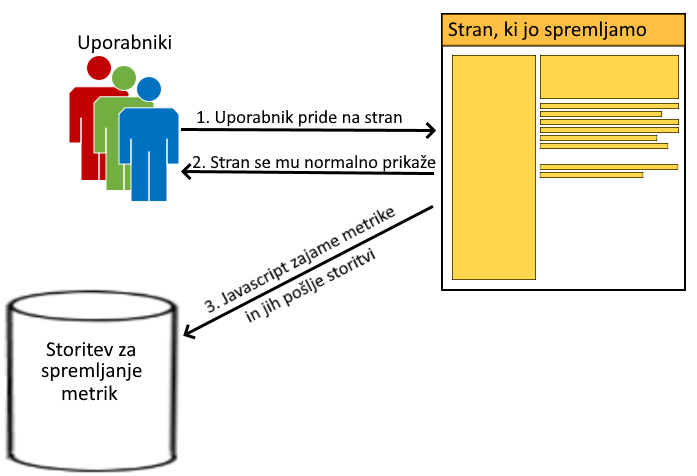
\includegraphics[width=0.9\textwidth]{rum_diagram.png}
	\end{center}
	\caption{Delovanje pasivnega spremljanja metrik}
	\label{img:rum}
\end{figure}

Ena od tehnologij pasivnega spremljanja je ti. spremljanje uporabniških metrik v realnem času (ang. Real User Monitoring, oziroma krajše RUM). S temi uporabniškimi metrikami, lahko nato zaznamo neželene pojave kot so pogoste napake ali upočasnitve. Zaznamo lahko odzivnost našega uporabniškega vmesnika, kjer spremljamo preklop med stanji aplikacije, pa tudi njegovo intuitivnost, tako, da spremljamo premik miške po zaslonu in vidimo, ali se uporabnik \sn{lovi} po zaslonu. Poleg tehničnih metrik, pa lahko spremljamo še ostale metrike, kot so število obiskov strani, ali se stranke vračajo na našo stran, kakšen čas v povprečju preživijo na njej, ipd.

Veliko teh metrik lahko spremljamo z uporabo orodij kot je Google Analytics \cite{ga_website} (nadalje GA) -- predvsem prej omenjene ne-tehnične metrike. GA je sicer orodje pisano za uporabo v klasičnih več-stranskih spletnih straneh, kjer se vsaka stran posebej naloži in takrat sproži dogodek, ki ga GA zabeleži, vendar lahko njegovo uporabo priredimo tako, da deluje tudi v enostranskih spletnih aplikacijah \cite{ga_spa}.

V primeru da želimo spremljati tehnične metrike naše enostranske spletne aplikacije, pa hitro ugotovimo, da nam GA ne zadošča. Tukaj je iniciativo prevzelo podjetje Microsoft, z razvojem orodja Mezzurite \cite{mezzurite_website}, (v času izdelave diplomske naloge je bila aplikacija verzije 1) ki ponuja zbiranje metrik za ogrodja Angular \cite{angular_website}, AngularJS \cite{angularjs_website} in React \cite{react_website}.

Pri tem je Microsoft naletel na problem, da so navigacija in življenjski cikel aplikacije zelo odvisni od ogrodja, ki ga uporabljamo. Predstavili so rešitev, kjer so podprli samo tri ogrodja in v zameno olajšali delo razvijalcu, ki uporablja njihov produkt. Dolgih nosov so tako ostali razvijalci, ki uporabljajo druga popularna ogrodja, npr. Vue.js \cite{vue_website}. Ker pa se popularnost ogrodij in tehnologij zelo hitro spreminja, je pri takem pristopu treba biti neprestano obveščen o spremembah in jih poznati v globino. Ogrodje je potrebno poznati  precej dobro, da vemo, kam umestiti naše spremljanje metrik. Tega se verjetno zaveda tudi Microsoft, saj je naznanil 2. verzijo platforme Mezzurite, kjer bo najverjetneje spremenil pristop.

V zasnovi razvite rešitve za spremljanje metrik, ki smo jo razvili v okviru diplomske naloge smo izbrali drugačen pristop kot Microsoft. Zasnovali smo generično rešitev, ki deluje neodvisno od uporabljenega ogrodja. Ta zahteva nekaj več dela s strani razvijalca in razvijalec mora poznati ogrodje, ki ga uporablja. Hkrati pa mu to omogoča, da prilagodi spremljanje metrik tako, da mu bo dalo karseda točne metrike, primerne za njegovo aplikacijo.

\chapter{Razlike pri spremljanju metrik enostranske spletne aplikacije (SPA) in klasične spletne strani}
\label{ch1}

Ker se enostranske spletne aplikacije razlikujejo v delovanju od klasičnih, se tako razlikuje tudi spremljanje metrik teh dveh pristopov \cite{spa_vs_multi} \cite{spa_blakit}. Merjenje metrik je v tem primeru, potrebno prilagoditi drugačnemu načinu delovanja, da nam dajo bolj točne podatke. Nekatere od teh sprememb pa potrebujejo tudi vpeljavo novih metrik, ki jih pri klasičnih straneh ne poznamo, saj pri SPA vplivajo na točnost spremljanih metrik.

\section{Pomembnost metrik v enostranskih spletnih aplikacijah}
\label{ch1:sec1}

Pri prehodu iz klasičnih strani na SPA se ne spremenijo samo metrike, ampak tudi njihova pomembnost. Klasične strani so večinoma pisane tako, da brskalnik prenese že zgrajeno stran in jo uporabniku samo prikaže, koda Javascript pa se samo odziva na dogodke, ki jih uporabnik proži – to so lahko kliki na gumb, ti. drag\&drop ali pa premik miške – in tako niso zahtevni za izvajanje. Pri SPA pa brskalnik prenese kodo Javascript, ki šele nato zgradi uporabniški vmesnik na odjemalčevi strani.

Izvajanje te kode pa se tukaj ne konča, saj velika večina teh ogrodij podpira tudi dvostransko vezavo podatkov (ang. two-way data binding) [Ilustrirano na sliki \ref{img:angularjs_two_way_databind}]. Torej, ko nek podatek v kodi zamenja vrednost (kot posledica rezultata klica AJAX, ali pa uporabniškega vnosa), se ta sprememba takoj pozna na vmesniku. Za dosego tega, je potrebno, da v ozadju koda neprestano posluša za spremembe ter, da prepozna, kdaj je potrebno vmesnik na novo izrisati. S tem koda v naši aplikaciji ni več pasivna, ampak deluje aktivno. To odpre pot možnim puščanjem pomnilnika ali pa upočasnitvam aplikacije.

\begin{figure}[h]
	\begin{center}
		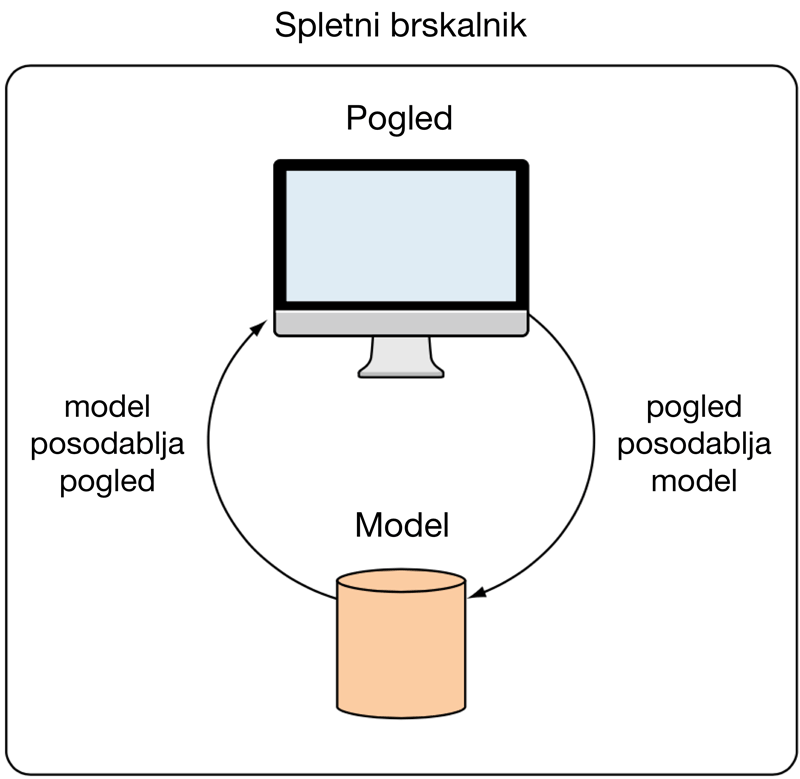
\includegraphics[width=0.9\textwidth]{AngularJS_dvosmerno_povezovanje.png}
	\end{center}
	\caption{Dvosmerno povezovanje pogleda in modela, vir: \cite{sp_skripta}}
	\label{img:angularjs_two_way_databind}
\end{figure}

Vse to naredi odjemalski del aplikacije precej bolj kompleksen v primerjavi s klasičnimi spletnimi stranmi. Pri obvladovanju kompleksnosti aplikacije nam pomagajo metrike, ki beležijo delovanje aplikacije. S temi metrikami lažje odkrivamo napake v naši aplikaciji, kar naredi spremljanje metrik zelo priporočljivo, če ne celo obvezno aktivnost.

\section{Metrike v enostranskih spletnih aplikacijah}
\label{ch1:sec2}

Ker je področje spremljanja metrik za SPA še precej novo, še nimamo poenotene terminologije za te metrike. Razne implementacije uporabljajo svojo terminologijo, vendar pa koncepti ostajajo isti \cite{linkedin_rum} \cite{mezzurite_website}.

Pri vseh implementacijah je moč najti zagonski čas aplikacije (ang. application load time, oziroma krajše ALT). To je metrika, ki nam pove, koliko časa potrebuje naša aplikacija, da prenese zahtevane gradnike, naloži kodo ogrodja, ki ga uporabljamo in inicializira aplikacijo. Gre za precej pomembno metriko, saj če je zagonski čas predolg, lahko izgubimo kakšnega potencialnega uporabnika. Občutek predolgega nalaganja se velikokrat zmanjša tako, da najprej prikažemo stran, ki uporabniku sporoči, da se stran nalaga – v večini primerov je to krog, ki se vrti, ali pa črta, ki se obarva glede na napredek (pomislimo na odjemalca Gmail, ki nas obvesti, da se aplikacija nalaga, nato pa prikaže vsebino) – ko smo pa prepričani, da je aplikacija naložena, to stran skrijemo in prikažemo dejansko vsebino. Eden izmed načinov je tudi ta, da se poslužimo delnega strežniškega upodabljanja (ang. server-side rendering), tj. da stran delno izrišemo že na strežniku.

Naslednja omembe vredna metrika se uporablja že pri klasičnih straneh. To je čas nalaganja strani (ang. page load time, oziroma krajše PLT). Pri klasičnih aplikacijah je to najpogostejša metrika, ki nas zanima, saj nam pove, kako hitro uporabnik vidi vsebino strani. Toda, ko skušamo to metriko vpeljati tudi v SPA, pridemo hitro do vprašanj, s katerimi se nismo srečali pri klasičnih straneh. Prvo vprašanje, ki se nam zastavi je, kdaj se stran sploh smatra za naloženo? Ali je to, ko se naloži DOM? Ali, ko se nam izriše vmesnik? Mogoče takrat, ko pridobimo podatke?

\begin{figure}[!htb]
	\begin{center}
		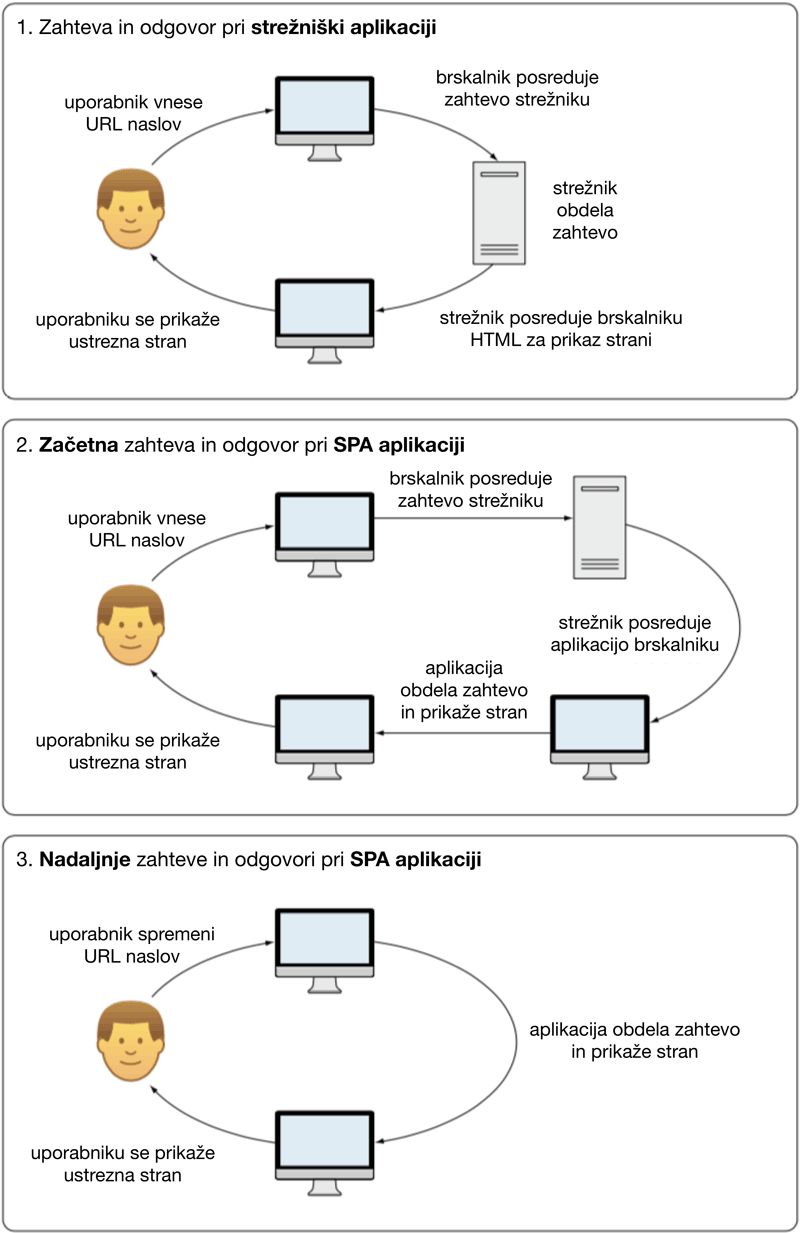
\includegraphics[width=0.9\textwidth]{Razlicni_nacini_obdelave_zahtev.png}
	\end{center}
	\caption{Različno delovanje SPA in klasičnih spletnih strani, vir: \cite{sp_skripta}}
	\label{img:diff_multipage_spa}
\end{figure}

Pravega odgovora ni, saj to povsem zavisi od tega, kako smo stran zasnovali. Tudi podatke, ki jih pridobivamo dinamično z zahtevki AJAX, ne obravnavamo z enako prioriteto. Podatki, ki gradijo osnovni pogled, na primer tabelo, so najverjetneje sestavni del strani in morajo biti zajeti v času nalaganja strani, medtem, ko podatek, ki nam prikazuje število neprebranih sporočil v orodni vrstici ni bistven in ga lahko iz te metrike izpustimo. V tem primeru mora razvijalec sam presoditi, kdaj je stran uporabna in se smatra kot naložena.

\FloatBarrier

\section{Razlike v navigaciji}
\label{ch1:sec3}

Poleg prej navedenega pa se enostranske spletne aplikacije razlikujejo tudi v navigaciji. Pri nalaganju posamezne strani se je potrebno vprašati, ali je ta stran prva, ki smo jo odprli, ali ena izmed sledečih? Namreč, kot je bilo že omenjeno, SPA se poslužujejo mehke navigacije [Slika \ref{img:diff_multipage_spa}]. To je navigacija, ki spremeni naslov URL in stanje zgodovine brskalnika z uporabo HTML5 history API-ja, brez, da bi se stran dejansko naložila. Posledica tega je, da je z izjemo prve, vsaka naslednja navigacija bistveno hitrejša. Torej če ne razlikujemo prve, \sn{trde} navigacije od ostalih, lahko  dobimo napačne podatke.

V čem pa se prva navigacija pravzaprav razlikuje od ostalih? Tukaj se spomnimo prej omenjenega zagonskega časa aplikacije. Ob prvi navigaciji se morajo prenesti gradniki aplikacije, nakar se mora aplikacija še inicializirati. Prva navigacija je zato sestavljena iz zagonskega časa aplikacije in časa nalaganja strani.

Zaradi tega dejstva hitro opazimo, da uporaba imena PLT pri SPA ni primerna. PLT pri klasičnih aplikacijah vsebuje tudi čas, ki ga porabimo da prenesemo gradnike strani, v primeru mehke navigacije, pa teh gradnikov ne prenašamo. To se zgodi samo v zagonskem času aplikacije. Zato je tukaj primernejše govoriti o času nalaganja pogleda (ang. view load time, oziroma krajše VLT). Prva navigacija je tako sestavljena iz dveh metrik, vsaka nadaljnja pa le iz ene.

\section{Posplošitev časa nalaganja strani v čas nalaganja komponente}
\label{ch1:sec4}

Pri večini SPA ogrodij so strani v bistvu samo komponente. Tako se vprašamo ali bi lahko čas nalaganja pogleda posplošili v čas nalaganja komponente (ang. component load time, oziroma krajše CLT)? Čeprav VLT in CLT izgledata kot, da merita isto stvar, pa vendar obstaja razlika med njima. VLT se prične meriti, ko se navigacija začne. V vsakem ogrodju je to drugače implementirano, ampak običajno se navigacija začne, ko smo še na prejšnji strani. V VLT tako zajamemo tudi čas, ki ga ogrodje porabi, da razreši katero komponento mora prikazati za zahtevan url.

Komponenta pa lahko pomeni tudi vnosno polje za datum -- ta komponenta ne bo imela svojega URL-ja, in bo lahko uporabljena na več straneh, ali pa celo večkrat na eni strani. Tukaj nas navigacija pravzaprav ne zanima, zanima nas samo koliko časa potrebuje komponenta, da se instancira in postane uporabna. Namesto na navigacijo, se tukaj zanašamo na življenjski cikel komponente. Vsaka komponenta ima, odvisno od ogrodja, definiran življenjski cikel, kjer se ustvari instanca komponente, izriše njen pogled, pridobi podatke, ki jih komponenta potrebuje in kjer se ta instanca izbriše iz spomina, ko je ne potrebujemo več.

To metriko je smiselno uporabiti na bolj kompleksnih komponentah, oziroma ti. \sn{pametnih} komponentah, ki znajo podatke pridobivati in obdelovati, da tako spremljamo njihovo učinkovitost. Pri \sn{neumnih} komponentah, tistih, ki znajo podatke samo prikazati, ne pa tudi pridobiti, pa najverjetneje ni.

Zaradi razlike v uporabi komponent, ki so pogledi in komponent, ki niso, je bolje, da čas nalaganja pogleda in čas nalaganja komponente obravnavamo in zajemamo ločeno.

\section{Smiselne metrike}
\label{ch1:sec5}

V enostranskih aplikacijah lahko spremljamo veliko število smiselnih metrik. Spodaj smo našteli nekaj metrik, ki se nam zdijo primerne za spremljanje v enostranskih aplikacijah, kljub temu pa nekatere izmed njih lahko uporabimo tudi pri klasičnih spletnih straneh. Nekaj od teh metrik smo tudi vključili v našo razvito rešitev.

\begin{description}
	\item[Čas nalaganja komponente:] O času nalaganja komponente smo govorili že v poglavju \ref{ch1:sec4}.
	\item[Beleženje poljubnih dogodkov:] S tem zajamemo število poljubnih enkratnih dogodkov, ki so se izvedli, kot so recimo izvedba neke akcije ali pa odpiranje zunanje povezave, kar nam da večji vpogled v to, za katere namene naši uporabniki uporabljajo našo aplikacijo in kako.
	\item[Spremljanje vračanja strank:] S hrambo stanja v internetnih piškotkih lahko spremljamo kolikokrat je uporabnik že obiskal našo stran iz neke naprave. Iz teh podatkov lahko sklepamo,  ali se stranke vračajo na našo stran. V primerih, ko imamo v aplikacijo vključeno še avtentikacijo, lahko spremljamo ali naši uporabniki dostopajo do aplikacije z različnimi napravami.
	\item[Spremljanje uporabniških naprav:] Velikokrat je smiselno spremljati tudi velikost zaslona in brskalnik. Tako lahko vidimo ali naši uporabniki pretežno uporabljajo mobilne naprave za dostop do aplikacije, kar pomeni, da moramo posvetiti več pozornosti odzivnemu uporabniškemu vmesniku.
	\item[Spremljanje časa uporabnika na strani:] Smiselno je beležiti tudi čas, ki ga uporabnik porabi na določeni strani. To še posebej drži za strani, katerih glavna funkcionalnost je prikazovanje vsebine, na primer razne novičarske strani, blogi ali forumi. Čeprav je veliko takih strani pisanih še kot klasične strani, pa so nekatere že pisane tudi kot enostranske spletne aplikacije. Spletni portal 24ur.com tako uporablja ogrodje Angular za prikaz novic. Obstajajo pa tudi razni generatorji statičnih strani, ki generirajo vsebino, posredujejo pa jo kot enostransko spletno aplikacijo, dva popularnejša sta Gatsby \cite{gatsby_website} in VuePress \cite{vuepress_website}. V kombinaciji s prej omenjenim beleženjem dogodkov, lahko dobimo res dobro sliko o kvaliteti naše storitve, ki jo uporabnikom ponujamo kot našo aplikacijo.
	\item[Spremljanje uporabnikove lokacije:] Spremljanje od kod naši uporabniki dostopajo do aplikacije je zelo pomembno. V primeru, da so naši strežniki preveč oddaljeni od naše glavne baze uporabnikov, jih je smiselno postaviti bližje.
	\item[Zagonski čas aplikacije:] Zajamemo čas, ki ga naša aplikacija potrebuje od začetka navigacije do trenutka, ko je naša aplikacija prenešena in inicializirana in se je pričela odzivati na zahteve uporabnika.
	\item[Čas nalaganja pogleda:] Čas, ki ga potrebuje aplikacija, da izriše novo stran (po tem, ko je aplikacija zagnana).
	\item[Čas nalaganja gradnikov strani:] Čas, ki ga gradniki strani potrebujejo, da se prenesejo. Ker ta čas zelo vpliva na zagonski čas aplikacije, ga je smiselno obravnavati posebej.
	\item[Spremljanje uporabe aplikacije:] Ker se v enostranskih aplikacijah stanje ohranja pri prehodu na novo stran, lahko spremljamo uporabo naše aplikacije tako, da sledimo poti, ki jo uporabnik gradi z odpiranjem novih strani naše aplikacije.
	\item[Spremljanje premikov miške:] Z zajemanjem premikov miške, lahko zaznamo razdalje, ki jih uporabnik \sn{prepotuje} z miško po ekranu. Ta podatek lahko potem vizualno prikažemo na vročinskem zemljevidu. Iz tega zemljevida lahko razberemo ali je možno te prepotovane razdalje optimizirati, da izboljšamo uporabniško izkušnjo.
\end{description}

Večina teh metrik je formalne narave, kjer ima metrika številčno vrednost in lahko na njej opravljamo statistično analizo. Iz tega se lahko razbere ali prihaja do problemov pri večjem deležu uporabnikov, ali pa le pri peščici.

Danes imamo namreč veliko spletnih standardov, ki jih ne podpirajo vsi brskalniki. To je sploh očitno pri uporabi starejših brskalnikov. Če iz zbranih podatkov razberemo, da ima nek določen problem samo peščica ljudi in to zaradi starejšega brskalnika, je mogoče cenejše opustiti podporo za ta brskalnik, kot pa prilagoditi aplikacijo zanj. Nedavno smo bili priča takemu primeru, ko je eden od popularnejših ponudnikov repozitorijev GIT, GitHub, sporočil novico, da so opustili podporo za brskalnik Internet Explorer [Slika \ref{img:github_ie}]

\begin{figure}[h]
	\begin{center}
		
\includegraphics[width=1\textwidth]{github_end_support.png}
	\end{center}
	\caption{Obvestilo na GitHub strani, odprti z Internet Explorerjem}
	\label{img:github_ie}
\end{figure}

Spremljamo pa lahko tudi metrike neformalne narave, kjer podatki nimajo neke številčne vrednosti, oziroma nam ta vrednost ne predstavlja neke dodane informacije. Tak primer je zajemanje premikov miške, kjer vidimo, kako intuitiven je naš vmesnik za uporabnika. Statistična analiza na teh podatkih nam ne bi prinesla ravno uporabnih podatkov, saj formula ne more vedeti, kako je naš uporabniški vmesnik zasnovan. V tem primeru, je bolj smiselno podatke evaluirati vizualno.

\chapter{Spremljane metrike v razviti rešitvi}
\label{ch2}

Metrik, ki jih lahko spremljamo pri spletnih aplikacijah, je veliko. Prav zaradi tega smo se pri implementaciji osredotočili le na nekaj izbranih metrik, ki dobro predstavijo proces zbiranja metrik.

\section{Problematika spremljanja metrik}

Čeprav je organizacija W3C predlagala standard, ki bi poenotil terminologijo in način zajemanja metrik (vidno na sliki \ref{img:w3c_metrics}), pa so te neprimerne za enostranske spletne aplikacije. To področje zaenkrat ostaja nestandardizirano, v veliki meri tudi zaradi obstoja velikega števila različnih ogrodij. Vsako ogrodje ima svoj življenski cikel komponent in svojo filozofijo delovanja.

\begin{figure}[h]
	\begin{center}
		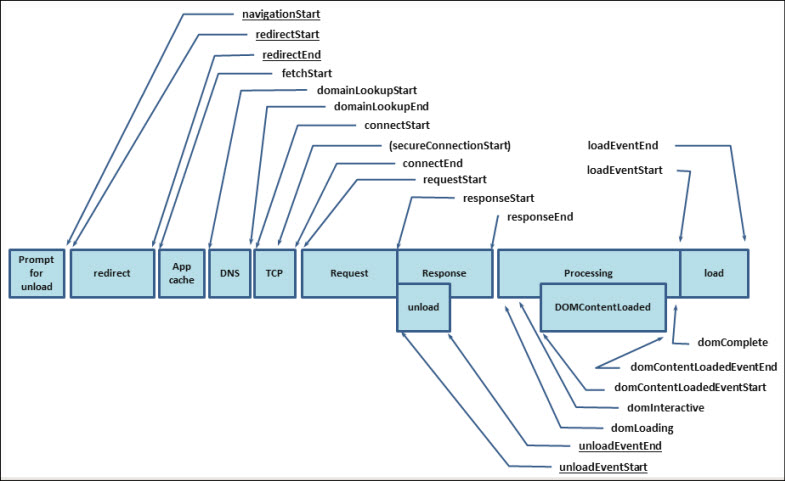
\includegraphics[width=1\textwidth]{w3c-metrics.jpg}
	\end{center}
	\caption{Predlog W3C za merjenje različnih časov nalaganja spletne strani}
	\label{img:w3c_metrics}
\end{figure}

Ko želimo spremljati metrike v enostranskih aplikacijah, hitro naletimo na problem, saj opazimo, da standardne metrike, ki jih predlaga W3C ne zadostujejo. Predlagani standard rešuje problematiko metrik pri klasičnih spletnih straneh, kjer je vsaka stran svoj dokument HTML. Stran smatra kot naloženo kmalu po tem, ko se naloži DOM. Ker pa mora enostranska aplikacija po inicializaciji objekta DOM, naložiti še svojo kodo, ta standard izpusti del časa nalaganja.

S tem ko so razvijalci skušali zajeti metrike, primerne za enostranske aplikacije, se je pojavilo veliko različnih implementacij zajemanja metrik. Vsaka implementacija uporablja svojo terminologijo in zajema metrike, ki niso standardne. V podjetjih, ki uporabljajo različne tehnologije, to lahko vodi v višje stroške usposabljanja razvijalcev, saj morajo poznati več različnih orodij in terminologijo, ki jo ta orodja uporabljajo.

Z našo zasnovano rešitvijo, se skušamo tem problemom izogniti, oziroma njihov učinek omiliti. Da bi to dosegli, smo razvili generično platformo, ki je neodvisna od uporabljenega ogrodja. To nam omogoča, da poenotimo terminologijo in interpretacijo podatkov.

\section{Zajemanje metrik}

Za zajemanje metrik smo uporabili različne funkcionalnosti, ki jih brskalnik in Javascript ponujata. Najpogosteje smo se pri zajemanju metrik poslužili razreda Date, s katerim smo zajeli čas ob določenem trenutku. To smo uporabili za merjenje zagonskega časa aplikacije in časa nalaganja pogleda. Pri merjenju zagonskega časa smo se poslužili uporabe HTML5 Performance API-ja. Ta izpostavi lastnost, ki hrani čas, ko je brskalnik pričel nalagati stran.

Problem pri HTML5 API-jih za metrike je ta, da standardizacija še poteka in tako niso zanesljivi. Veliko jih je tudi v opuščanju, ker je v pripravi boljši predlog. Brskalnik Chrome, ki ga izdeluje podjetje Google, ponuja veliko eksperimentalnih API-jev, ki pa so lahko stvar spremembe ali pa ne delujejo zanesljivo. Ker pa so implementirani samo v Chromeu, pomeni, da metrike zajete s temi API-ji izključijo segment naših uporabnikov (teh, ki ne uporabljajo Chroma) in tako lahko vplivajo na kvaliteto naših podatkov.

Izjemo smo naredili za eno lastnost Performance API-ja in sicer objekt PerformanceTiming, ki nam izpostavi lastnost navigationStart. Ta lastnost je v opuščanju, vendar jo večina brskalnikov še vedno podpira. Kot nadomestilo te lastnosti se uvaja lastnost Performance objekta timeOrigin, ki pa ni še standardizirana. V našem pristopu tako preverjamo, če je timeOrigin definiran in če ni, uporabimo opuščeni PerformanceTiming objekt.

Uporabili smo še poslušalca dogodka (ang. event listener) premika miške. Ta posluša za spremembo položaja miške in ob spremembi zabeleži novo pozicijo miške.

\section{Zajete metrike}
\label{ch2:sec0}

Izmed metrik, ki so se nam zdele smiselne za spremljanje (opisane v poglavju \ref{ch1:sec5}), smo jih nekaj izbrali in njihovo spremljanje implementirali v naši razviti rešitvi. Pri odločitvi katere metrike bomo zajemali smo uporabili lastno presojo, katere metrike najbolje ponazorijo spremljanje metrik v enostranskih spletnih aplikacijah.

\subsection{Zagonski čas aplikacije}
\label{ch2:sec1}
Ta metrika nam pove koliko časa potrebuje naša aplikacija od trenutka, ko v naslovno vrstico vnesemo spletni naslov aplikacije in pritisnemo ENTER, pa do prve navigacije na naši strani. Za označbo te metrike se uporablja angleška kratica ALT – Application Load Time.

Metriko zajemamo s pomočjo HTML5 Performance API-ja. Ta API nam izpostavi začetni čas navigacije, tj. ko smo pritisnili tipko ENTER, oziroma kliknili na povezavo, ki kaže na našo aplikacijo. Ta začetni čas pridobimo s klicem \verb|performance.timing.navigationStart| (uporaba v opuščanju) oziroma, z novejšim \verb|performance.timeOrigin|. Vse kar mora razvijalec narediti, da prične beležiti metriko je, da na primernem mestu pokliče metodo objekta MetricsMonitor iz naše razvite rešitve za spremljanje metrik, \verb|MetricsMonitor.logApplicationStartup()|, ki zabeleži trenutni čas, tj. konec zagona aplikacije in ta podatek posreduje naši storitvi za spremljanje metrik, ki ta podatek shrani.

\begin{lstlisting}[label=code:app_startup_report, caption=Poročilo zagonskega časa aplikacije]
{
  "minLoadTime": 124,
  "maxLoadTime": 2616,
  "avgLoadTime": 417.30232558139534,
  "percentiles": [
    {
      "percentile": 0.95,
      "value": 1598.6999999999985
    }
  ]
}
\end{lstlisting}

Ob zadostnem številu zbranih podatkov, si lahko ogledamo poročilo zagonskega časa, ki ga storitev za spremljanje metrik izpostavi preko REST API-ja (primer poročila je viden v izseku kode \ref{code:app_startup_report}).


\subsection{Čas nalaganja pogleda}
\label{ch2:sec2}

Čas nalaganja pogleda je čas, ki ga aplikacija porabi od klika na povezavo, do trenutka, ko vidimo vsebino zahtevane strani. Kaj se smatra kot vsebino strani je subjektivno, saj se to razlikuje od aplikacije do aplikacije. V takem primeru je to odločitev najbolje prepustiti razvijalcu, saj najbolje pozna aplikacijo. Za označbo te metrike se uporablja kratica VLT – View Load Time.

Posebej je potrebno izpostaviti čas nalaganja prvega pogleda (ang. first view load time, oziroma krajše FVLT). Ta čas dobimo tako, da seštejemo zagonski čas aplikacije in čas nalaganja pogleda (enačba \ref{eq:fvlt}).

\begin{equation}
\label{eq:fvlt}
FVLT = ALT + VLT
\end{equation}

Pomembno je, da ko merimo hitrost nalaganja posamezne strani (z VLT metriko), pri tej ne upoštevamo FVLT, saj tako lahko pokvarimo zajete podatke. Če na to nismo pozorni, se lahko hitro zgodi, da nam metrika pokaže, da je naša naslovna stran najpočasnejša, kar pa ni vedno res, lahko je le najpogostejša stran, ki jo uporabnik prvo obišče.

Za beleženje te metrike ne potrebujemo nobenega posebnega HTML5 API-ja, saj se metrika zajema, ko je DOM že v celoti naložen in nam tako razred \verb|Date| povsem zadostuje. Razvijalec v tem primeru uporabi dve metodi in sicer \verb|MetricsMonitor.logPageLoadStart(url)| in \\ \verb|MetricsMonitor.logPageLoadEnd(url)|. Metrika se shranjuje pod unikatnim imenom, da jo lahko razberemo od ostalih. Za unikatno ime je priporočljivo uporabiti kar URL strani. Isto metodo pa lahko uporabimo tudi za merjenje CLT posamezne komponente – tam uporabimo neko drugo, smiselno ime.
 
Enako kot pri zagonskem času aplikacije, nam storitev za spremljanje metrik izpostavi poročilo te metrike preko REST vmesnika (primer v izseku kode \ref{code:page_load_report}).

\begin{lstlisting}[label=code:page_load_report, caption=Poročilo časa nalaganja pogleda]
{
  "pages": [
    {
      "pathname": "/",
      "minLoadTime": 25,
      "maxLoadTime": 341,
      "avgLoadTime": 69.04347826086956,
      "pageHits": 23,
      "percentiles": [
        {
          "percentile": 0.95,
          "value": 120.1
        }
      ]
    },
    {
      "pathname": "/service/{id}",
      "minLoadTime": 26,
      "maxLoadTime": 295,
      "avgLoadTime": 72.18518518518519,
      "pageHits": 27,
      "percentiles": [
        {
          "percentile": 0.95,
          "value": 212.49999999999997
        }
      ]
    }
  ],
  "averagePageLoadTime": 69.43939393939394
}
\end{lstlisting}

Poročilo nam za vsako stran izpiše minimalni, maksimalni in povprečni čas nalaganja, število kolikokrat je bila ta stran obiskana in percentile, ki jih lahko poljubno specificiramo s parametri zahtevka. Storitev za spremljanje metrik ponuja še en dodatni parameter, s katerim ji lahko povemo naj v poročilo vključi tudi FVLT, ne samo VLT.

V poročilu [Izvorna koda \ref{code:page_load_report}] pričakovano dobimo zelo kratke čase nalaganja pogleda, saj je navigacija v enostranskih spletnih aplikacijah precej hitra.

\subsection{Čas nalaganja gradnikov strani}
\label{ch2:sec3}

Velik delež zagonskega časa aplikacije normalno predstavlja nalaganje gradnikov strani. To so datoteke, ki jih naša aplikacija nujno potrebuje za svoje delovanje in so lahko različnega tipa, najpogosteje pa s tem mislimo na HTML, Javascript in CSS datoteke.

To metriko je smiselno spremljati zato, da lahko zaznamo ali imajo uporabniki težave s prenašanjem delov naše aplikacije na njihove naprave. Seveda je prenos aplikacije odvisen od kvalitete internetne povezave našega uporabnika, to pa je faktor na katerega nimamo vpliva.

V kolikor prepoznamo, da ima znaten del naših uporabnikov težave s prenašanjem, se poslužimo raznih tehnik, ki naredijo našo aplikacijo bolj vitko. V kombinaciji z ostalimi metrikami lahko zaznamo, da določena sekcija naše aplikacije ni tako obiskana kot ostale -- recimo urejanje profila. Tako sekcijo je zato smiselno naložiti s ti. lenim nalaganjem (ang. lazy loading), s čimer zmanjšamo zagonski čas aplikacije.

Za zajem te metrike se spet poslužimo HTML5 Performance API-ja. Ob zagonu aplikacije, se sproži koda, ki s klicem \\ \verb|performance.getEntriesByType("resource")| odčita čase nalaganja posameznega gradnika ter njegovo velikost. Posamezen gradnik ima več časov nalaganja. API nam izpostavi čase preusmeritve, DNS razrešitve, vzpostavitve povezave TCP, rokovanja SSL/TLS. Iz izpostavljenih lastnosti, pa lahko izračunamo še začetek zahtevka in konec odgovora, iz katerega lahko dobimo celoten čas prenosa. API nam tudi izpostavi velikost prenešene datoteke in velikost odgovora na zahtevek HTTP. To nam omogoča, da vidimo koliko bajtov podatkov je uporabnik dejansko prenesel.

Ta metoda ima en pomemben predpogoj in sicer mora strežnik, ki streže te datoteke implementirati glavo zahtevka HTTP Time-Allow-Origin, kjer za vrednost podamo domene, iz katerih je zbiranje te metrike dovoljeno. Delovanje je tako podobno CORS-u.

Tudi pri tej metriki, nam storitev za spremljanje metrik izpostavi poročilo preko REST vmesnika (primer v izseku kode \ref{code:resource_load_report}).

\begin{lstlisting}[label=code:resource_load_report, caption=Poročilo časa nalaganja gradnikov strani]
{
  "resources": [
    {
      "name": "http://192.168.1.22:32772
        /styles.6b7abb61d8006c2e7e17.css",
      "type": "link",
      "payloadSize": {
        "average": 245425.0,
        "minimum": 245425,
        "maximum": 245425
      },
      "requestSize": {
        "average": 52837.78571428572,
        "minimum": 224,
        "maximum": 245755
      },
      "requestTime": {
        "average": 39.035714285714285,
        "minimum": 2,
        "maximum": 562
      }
    },
    {
      "name": "http://192.168.1.22:32771
        /main.86563ff2a46d83c7aa1d.js",
      "type": "script",
      "payloadSize": {
        "average": 1642994.0,
        "minimum": 1642994,
        "maximum": 1642994
      },
      "requestSize": {
        "average": 1643339.0,
        "minimum": 1643339,
        "maximum": 1643339
      },
      "requestTime": {
        "average": 218.5,
        "minimum": 163,
        "maximum": 326
      }
    }
  ]
}
\end{lstlisting}

Poročilo nam za vsak gradnik posebej izpiše njegov tip, minimalno in maksimalno ter povprečno vrednost za tri metrike: velikost datoteke, velikost HTTP zahtevka (ki poleg datoteke vsebuje še meta podatke kot so HTTP glave -- ang. HTTP headers) in čas, ki je bil potreben, da se je datoteka prenesla.

\subsection{Sledenje premikov miške uporabnika}
\label{ch2:sec4}

Sledenje premikov miške je še zadnja od metrik, ki smo jih zajeli v razviti rešitvi. Za razliko od preostalih, nam ta ne meri hitrosti naše aplikacije, ampak jo uporabljamo, da ugotavljamo intuitivnost našega uporabniškega vmesnika. Ker ni formalne narave, ne moremo podatkov spraviti v neko številsko obliko in jih prikazati v poročilu, kot smo to storili s prejšnjimi metrikami \cite{ux_book}.

Seveda, pa to ne pomeni, da so taki podatki nekoristni. Če te podatke združimo v skupine pikslov (npr. 20px x 20px), lahko za vsako tako skupino beležimo ti. vročinsko stopnjo. Ta stopnja nam predstavlja število kolikokrat je uporabnik šel z miško čez to skupino pikslov. Skupine pikslov, ki so okoli gumbov bodo tako imele višjo vročinsko stopnjo, kot tiste v robovih aplikacije, kjer običajno ni vsebine.

Ko imamo izračunane vročinske stopnje, lahko s temi stopnjami izrišemo vročinski zemljevid naše aplikacije. Za izris zemljevida, moramo spremeniti način delovanja odjemalca iz zajemanja metrik v risanje vročinskega zemljevida. Odjemalec bo tako pridobil podatke potrebne za izris, in jih izrisal na zaslon poleg naše aplikacije, kot je to vidno na sliki \ref{img:heatmap}. Pri tem bodo polja z višjo vročinsko stopnjo obarvana temnejše (rdeče), polja z nižjo pa svetlejše (zeleno).

\begin{figure}[h]
	\begin{center}
		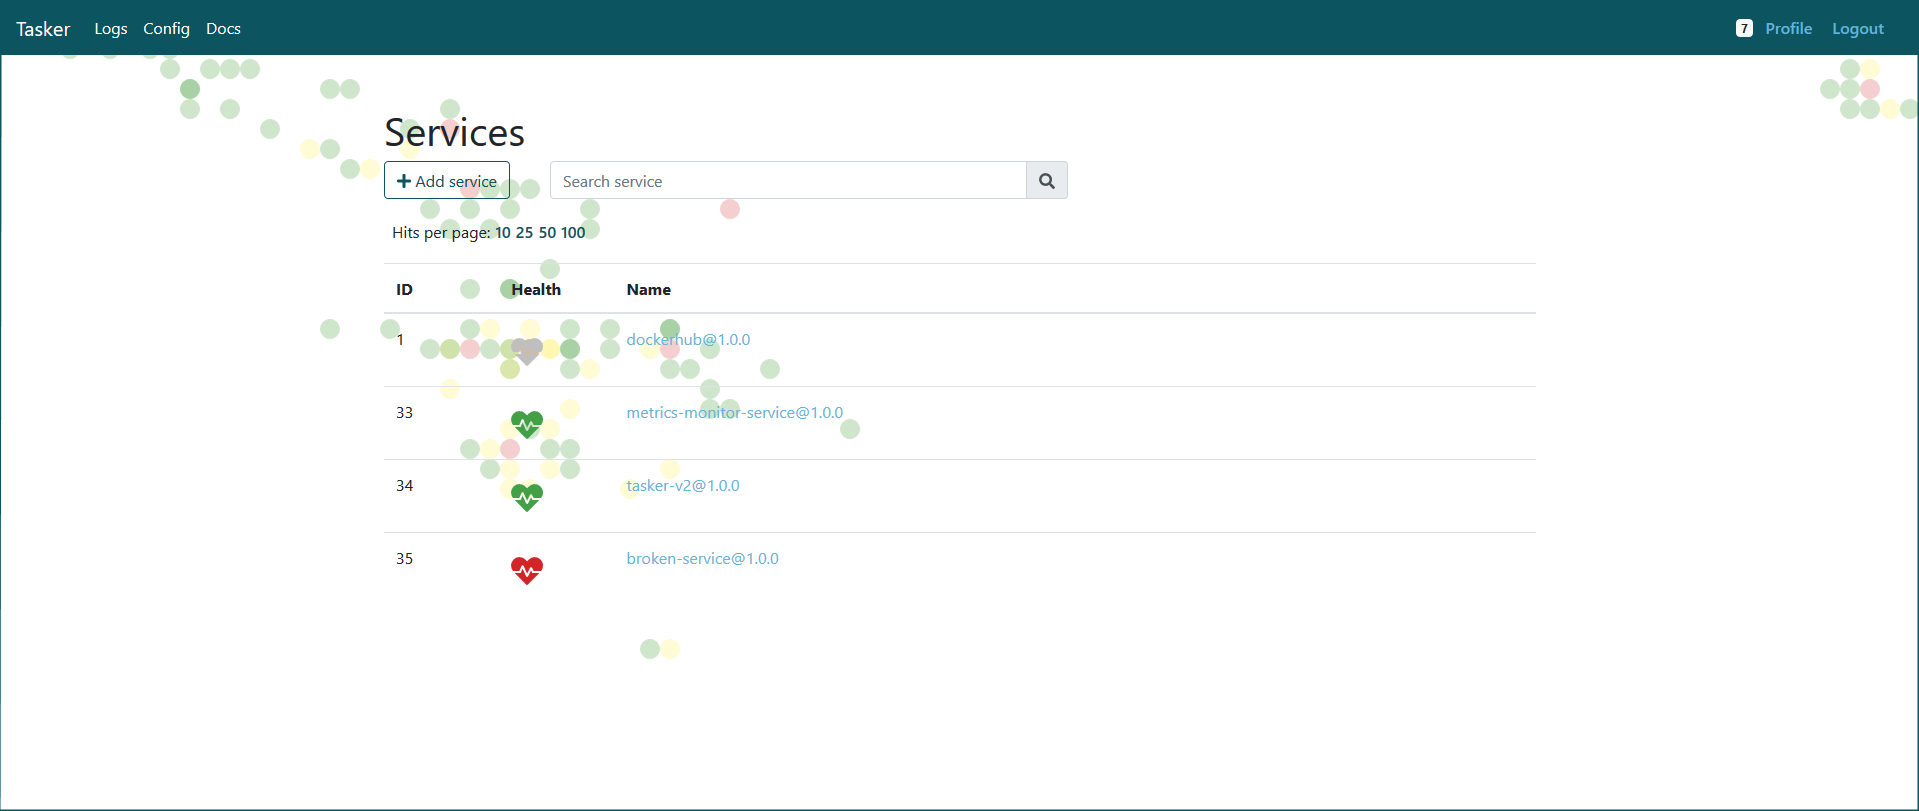
\includegraphics[width=1\textwidth]{heatmap_1.png}
	\end{center}
	\caption{Primer vročinskega zemljevida}
	\label{img:heatmap}
\end{figure}

Iz izrisanega vročinskega zemljevida lahko na neformalen način vidimo, ali se naši uporabniki preveč \sn{lovijo} po zaslonu, iz česar lahko sklepamo, da naš uporabniški vmesnik ni intuitiven. Vidimo pa lahko tudi množice najpogostejših akcij, ki jih uporabnik izbere. Če so gumbi za te akcije preveč oddaljeni med seboj, bo tako vročinski zemljevid izrisal pot med njimi, kar nam da informacijo, da je mogoče smiselno te gumbe premakniti bližje drug drugemu.

\chapter{Zasnova generične rešitve za zbiranje in spremljanje uporabniških metrik}
\label{ch3}

Za zajemanje metrik, opisanih v poglavju \ref{ch2:sec0}, smo zasnovali in razvili prototip platforme. V nadaljevanju opišemo zasnovo razvite platforme in njene komponente. Nato opišemo kako smo platformo implementirali in katera orodja smo pri tem uporabili. Demonstriramo še njeno uporabo v dejanski aplikaciji in nakažemo interpretacijo podatkov.

\section{Načrt razvite rešitve}
\label{ch3:sec1}

Pri snovanju rešitve za zbiranje uporabniških metrik v realnem času moramo biti še posebej pozorni, da z zbiranjem metrik ne poslabšamo uporabniške izkušnje naših uporabnikov. Pri takem zbiranju podatkov, je lahko uporabnikov aplikacije zelo veliko. Če se naša storitev za spremljanje metrik, ki metrike shranjuje, ne obnese dovolj dobro pri velikem številu zahtevkov, potem to lahko upočasni našo aplikacijo, katere metrike spremljamo.

Naših uporabnikov pa te metrike ne zanimajo, njih zanima samo storitev, ki jo naša aplikacija ponuja. V primeru, da imamo počasno aplikacijo, bodo uporabo naše aplikacije opustili in odšli h konkurenci. Najboljša rešitev za spremljanje metrik je torej taka, za katero uporabnik ne ve, ne da bi prebral ustrezna obvestila (na primer opozorilo na piškotke ali nova določila GDPR).

Metrike zajema knjižnica, ki jo vključimo v aplikacijo, katero želimo spremljati. Ta knjižnica odpre povezavo s storitvijo za spremljanje metrik, ki je del razvite rešitve, preko protokola WebSocket. Povezava se tako vzpostavi samo enkrat in ostane odprta dokler uporabnik uporablja aplikacijo. Preko te povezave nato pošiljamo zajete metrike. Nekatere metrike, kot so časi nalaganja se prenesejo takoj, medtem ko se premiki miške shranjujejo v medpomnilnik in se na vsakih nekaj zapisov prenesejo v storitev za spremljanje metrik, da se tako zmanjša število poslanih sporočil. Ko ta sporočila prispejo na strežnik, jih ta takoj umesti v sporočilno vrsto.

Iz tega razloga smo v zasnovo vključili Apache Kafko, platformo za distribuirano pretakanje. V platformi prevzema vlogo sporočilne vrste in s tem omogoča kasnejše procesiranje prejetih metrik. Kafka za svoje delovanje potrebuje tudi konfiguracijski strežnik Zookeeper. Drugi del storitve za spremljanje metrik jemlje sporočila iz vrste in jih glede na njihov tip ustrezno procesira ter shrani v podatkovno bazo. Ta del je lahko počasnejši, saj na delovanje spremljane aplikacije nima vpliva. Če se izkaže, da sprejemanje in procesiranje sporočil v isti storitvi slabo vpliva na optimalno delovanje le-te, se jo lahko loči na dva dela. Ima pa storitev za spremljanje metrik še tretjo komponento in to je generiranje poročil o zajetih metrikah. Ta del storitve, združi shranjene podatke in jih v JSON obliki posreduje razvijalcu.

Vse komponente platforme je moč videti na sliki \ref{img:design}. Spremljana aplikacija pridobiva podatke za svoje delovanje iz številnih API-jev. V ozadju spremljane aplikacije naša knjižnica spremlja metrike in jih pošilja storitvi za spremljanje metrik. Ta storitev sporočilo potisne v sporočilno vrsto v Kafki. Kafka za odkrivanje svojih preostalih instanc uporablja Zookeeper. Storitev nato odjema sporočila iz vrste in jih procesira.

\begin{figure}[h]
	\begin{center}
		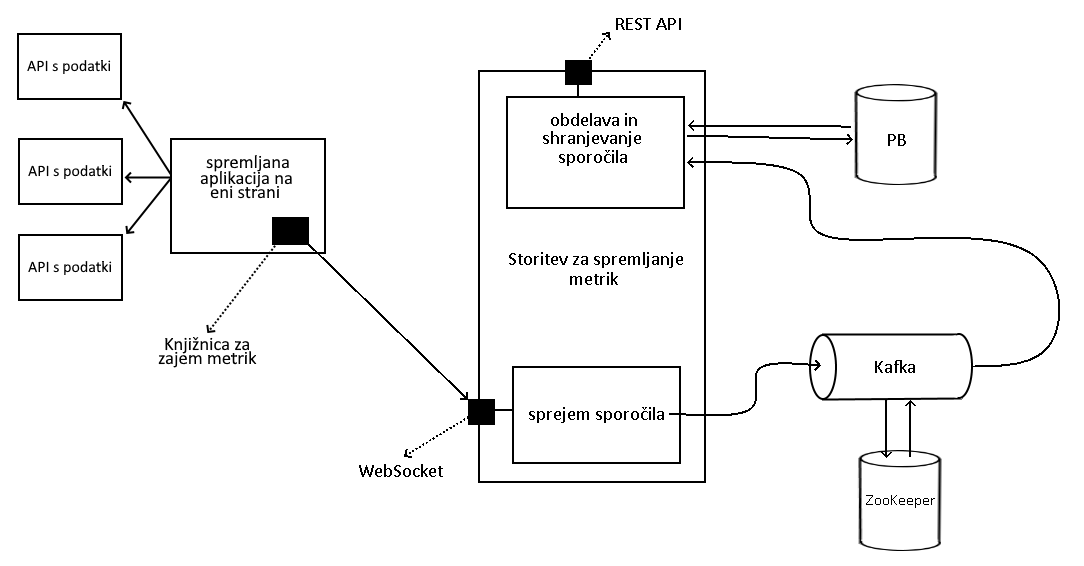
\includegraphics[width=1\textwidth]{design.png}
	\end{center}
	\caption{Načrt platforme}
	\label{img:design}
\end{figure}

Cilj te naloge je bil izdelati generično rešitev. Torej rešitev, ki je neodvisna od (ne)uporabljenega ogrodja. Da bi rešitev bila res generična se pri implementaciji knjižnice za zajem metrik, nismo poslužili nikakršnih optimizacijskih trikov, ki jih ogrodja prinašajo.

V drugem poglavju omenjen Mezzurite, je naredil prav to. Izkoristili so poznavanje delovanja ogrodja tako, da so napisali knjižnico, ki posluša dogodke v življenjskem ciklu in izvaja beleženje ob primernih trenutkih. Ker pa taka rešitev ni generična, smo mi izbrali drugačen pristop.

V knjižnici za spremljanje metrik tako samo izpostavimo metode, katere mora razvijalec ustrezno umestiti v aplikacijo. Torej mora te poslušalce dogodkov sam implementirati, iz česar sledi, da mora tudi poznati življenjski cikel ogrodja, ki ga uporablja.

Pri shranjevanju podatkov o metrikah pa je izstopalo shranjevanje premikov miške, saj je teh podatkov lahko zelo veliko. Pri Full HD zaslonu imamo 1920 x 1080 pikslov, zaradi česar bi hranjenje vsakega piksla pomenilo zelo veliko shranjenih vrstic v bazi. Za izris vročinskega zemljevida pa pravzaprav ne potrebujemo podatkov natančnih na en piksel, saj so ugotovitve iz zemljevida neformalne narave. Zato, da se izognemo temu problemu, smo piksle združevali v skupine 20x20 pikslov. S tem smo zmanjšali hranjeno mrežo iz 1920 x 1080 na 96 x 54, torej smo zmanjšali število hranjenih vrstic iz dobrih dveh milijonov na približno pet tisoč vrstic.

\section{Implementacija}
\label{ch3:sec2}

Za prototip generične rešitve je bilo potrebno implementirati spletno storitev za spremljanje metrik, ki metrike shranjuje in knjižnico, ki te metrike zajema in posreduje storitvi za spremljanje metrik.

\subsection{Knjižnica za zajem metrik}
\label{ch3:sec2:sub1}

Čeprav je Javascript še vedno edini jezik, ki ga brskalniki podpirajo, pa danes poznamo veliko načinov za pisanje spletnih aplikacij. Kot de facto standard za distribucijo spletnih aplikacij se uporablja ECMAScript 5 verzijo Javascripta. Ker je pa to zelo star standard, praktično noben razvijalec ne uporablja več te verzije. Tako je najpogostejši proces tak, da pišemo našo aplikacijo v novejši verziji Javascripta (ta je trenutno ES10, oziroma ECMAScript 2019), nato pa uporabimo prevajalnik (ang. transpiler), ki prevede kodo na starejšo verzijo. Najpopularnejši prevajalnik Javascript je trenutno Babel.

Ni pa to edini način, ki se danes uporablja za razvoj aplikacij. Microsoft je razveselil velik del razvijalcev, ko je zasnoval TypeScript, jezik enak Javascriptu, ki pa v koraku prevajanja preveri tudi podatkovne tipe spremenljivk in nam tako ponudi statično preverjanje tipov.

Ker imamo več različnih načinov razvoja, pa imamo tudi več načinov nalaganja modulov (oziroma datotek in knjižnic) v našo aplikacijo \cite{js_modules}. CommonJS, AMD in UMD so le eni izmed njih. UMD, ki je kombinacija prvih dveh, nam ponuja največjo fleksibilnost pri uporabi, zato smo se odločili napisati knjižnico v tem modulskem sistemu.

Knjižnico za zajem metrik smo pisali v prej omenjenem Typescriptu, ker dokumentiranje tipov, ki ga Typescript ponuja, omogoča lažjo uporabo knjižnice. Dodatno prednost predstavlja tudi dejstvo, da v primeru, ko uporabnik knjižnice uporablja samo Javascript, znajo moderni urejevalniki prebrati definicijo tipov in tako boljše predlagati uporabo knjižnice uporabniku.

V primerih, ko knjižnico za zajem metrik vključimo v aplikacijo z elementom \verb|<script>|, pa je pomembno tudi, da je ta knjižnica karseda majhna, da se hitreje naloži. Da to dosežemo se pri prevajanju izvede dodaten korak, minifikacija, ki kodo optimizira, odstrani neuporabljene dele kode in tako lahko zmanjša velikost knjižnice tudi za več kot 50 \%.

Vse te korake smo avtomatizirali z uporabo orodja Webpack, ki preko vtičnikov omogoča izvedbo celotnega prevajalnega cikla z enim ukazom. 

Prevedeno knjižnico smo nato namestili v zaseben repozitorij NPM, gostovan na Sonatypovem Nexusu, od koder smo nato knjižnico prenašali za uporabo v testnih aplikacijah.

\subsubsection{Delovanje knjižnice}

Ob zagonu knjižnica preveri zdravje storitve za spremljanje metrik na katero bo pošiljala podatke. Če je storitev v dobrem zdravju, odpre povezavo s protokolom WebSocket [Izvorna koda \ref{code:socket_conn}]. Ko je povezava vzpostavljena, knjižnica zaprosi storitev za pričetek seje. Pričetek seje storitev potrdi tako, da vrne enolični identifikator seje, ki se doda vsem naslednjim sporočilom, ki jih knjižnica pošilja. Knjižnica ustvari še interval, ki vsako minuto osveži povezavo s storitvijo, saj jo storitev v nasprotnem primeru zapre zaradi pomanjkanja aktivnosti.

\begin{lstlisting}[label=code:socket_conn, caption=Odpiranje WebSocket povezave in metode za upravljanje WebSocket akcij]
public static connectSocket(serverUrl: string): Promise> {
  return new Promise((resolve, reject) => {
    const socketUrl = (serverUrl + SOCKET_ENDPOINT)
        .replace("http", "ws");
    SocketService.socket = new WebSocket(socketUrl);

    SocketService.socket.onerror = (e: Event) => {
      MonitorState.getMonitorState().socketConnected = false;
      reject(new Error("Connection to socket failed!"));
    };

    SocketService.socket.onopen = (e: Event) => {
      MonitorState.getMonitorState().socketConnected = true;
      // pridobi identifikator seje
      SocketService.sendRegistrationEvent();
      // vsako minuto posljemo signal strezniku,
      // da ne prekine povezave zaradi neaktivnosti
      SocketService.intervalID = setInterval(
          SocketService.pingServerSocket,
          60000
      );
      resolve();
    };
    // ... 
  });
}

public static sendMessage(message: SocketMessage): void {
  if (SocketService.socket.readyState === SocketService.socket.OPEN) {
    SocketService.socket.send(JSON.stringify(message));
  }
}

private static onSocketMessage(e: MessageEvent): void {
  try {
    const message: SocketMessage = Object.assign(
        new SocketMessage(),
        JSON.parse(e.data)
    );
    SocketHandlerService.handleSocketMessage(message);
  } catch (e) {
    Logger.error("Error parsing socket message." +
        " Message must be valid JSON!");
  }
}
\end{lstlisting}

Ko imamo vpostavljeno povezavo, lahko pričnemo z zbiranjem metrik. Ko se bo sprožila metoda za beleženje zagonskega časa, bomo zajeli začetni čas navigacije in trenutni čas ter ju posredovali storitvi za spremljanje metrik. V naši metodi za zajem prvo zabeležimo trenutni čas, da se s tem izognemo latenci vzpostavitve povezave [Izvorna koda \ref{code:app_startup_tracker}].

\begin{lstlisting}[label=code:app_startup_tracker, caption=Zajemanje zagonskega časa aplikacije]
public static trackApplicationStartup() {
  // zajem koncnega casa
  const applicationLoaded = Date.now();
  // ce API ni na voljo, ne moremo zajemati metrike
  if (!AppStartupTracker.isFeatureEnabled()) {
    return;
  }

  if (MonitorState.getMonitorState().startingApplication) {
    // zajem zacetnega casa metrike z
    // uporabo Performance API-ja
    let navigationStart: number;
    if (MonitorState.getMonitorState()
        .browserFeatures["timeOrigin"]) {
      navigationStart = performance.timeOrigin;
    } else if (MonitorState.getMonitorState()
        .browserFeatures["navigationStart"]) {
      navigationStart = performance.timing.navigationStart;
    }

    MonitorState.getMonitorState().setStartedApplication();
    // ker se ta klic lahko izvede prej kot smo
    // vzpostavili WebSocket povezavo,
    // pocakamo na dodeljeno sejo
    execSessionFunc(() => {
      const message = new AppStartupMessage();
      message.applicationLoaded = applicationLoaded;
      message.navigationStart = navigationStart;
      SocketService.sendMessage(message);
    });
    // zabelezimo prenesene gradnike strani
    ResourceTracker.trackResources();
  }
}

private static isFeatureEnabled(): boolean {
  return MonitorState.getMonitorState()
      .browserFeatures["timeOrigin"] ||
    MonitorState.getMonitorState()
      .browserFeatures["navigationStart"];
}
\end{lstlisting}

V izvorna kodi \ref{code:app_startup_tracker} je moč opaziti klic metode za spremljanje gradnikov strani. Ta metoda zajame podatke o gradnikih, ki jih vmesnik PerformanceResourceTiming izpostavi in jih posreduje storitvi za spremljanje metrik [Izvorna koda \ref{code:resource_tracker}]. 

\begin{lstlisting}[label=code:resource_tracker, caption=Zajemanje gradnikov aplikacije]
public static trackResources(): void {
  if (MonitorState.getMonitorState()
      .browserFeatures["entriesByType"]) {
    // pridobimo vse gradnike
    const entries: PerformanceEntryList = performance
        .getEntriesByType("resource");
    entries.forEach((entry: PerformanceEntry) => {
      const resourceEntry = entry as PerformanceResourceTiming;
      execSessionFunc(() => {
        const message = ResourceTracker
            .collectEntry(resourceEntry);
        SocketService.sendMessage(message);
      });
    });
  }
}
\end{lstlisting}

Zajeti je potrebno še sledenje miški uporabnika. To dosežemo s poslušalcem dogodka premika miške [Izvorna koda \ref{code:mouse_tracker}]. Poslušamo dogodek \sn{mousemove}, ki se sproži vsakič, ko miškin kazalec spremeni koordinate. Te koordinate se shranjujejo v medpomnilnik -- ko se ta napolni, posredujemo njegovo vsebino storitvi za spremljanje metrik.

\begin{lstlisting}[label=code:mouse_tracker, caption=Spremljanje premikov miške]
public static registerMouseTracker(bufferLimit: number = 10) {
  MouseTracker.BUFFER_LIMIT = bufferLimit;
  MouseTracker.BUFFER = [];
  window.addEventListener(
      "mousemove",
      MouseTracker.onMouseTrack
  );
}

private static onMouseTrack(e: MouseEvent): void {
  // zajemamo dokler se medpomnilnik ne napolni
  if (MouseTracker.BUFFER.length < 
      MouseTracker.BUFFER_LIMIT) {
    const record: MouseRecord = {
      pageX: e.pageX,
      pageY: e.pageY,
      pathname: UrlUtil.getCurrentPathname(),
    };
    MouseTracker.BUFFER.push(record);
  } else {
    // ko je medpomnilnik poln, posljemo podatke storitvi
    const mouseTrackMessage = new MouseTrackMessage();
    mouseTrackMessage.coordinates = MouseTracker.BUFFER;
    SocketService.sendMessage(mouseTrackMessage);
    MouseTracker.BUFFER = [];
  }
}
\end{lstlisting} 

\subsection{Storitev za spremljanje metrik}
\label{ch3:sec2:sub2}

Storitev za spremljanje metrik smo razvijali v platformi Open JDK Java 11, pri čemer smo uporabili spletno ogrodje KumuluzEE, ki implementira specifikacije JakartaEE (oz. JavaEE 8) in MicroProfile 2.2. Ogrodje je bilo sprva razvito kot rezultat diplomske naloge \cite{kumuluz_diploma}. Ena od prednosti uporabe tega ogrodja je ta, da našo kodo zapakira v eno samo datoteko JAR, pogosto imenovano Fat Jar oziroma Uber Jar. V to datoteko nam vključi tudi strežnik Jetty, kar nam precej olajša namestitev programa, saj nam ni potrebno konfigurirati aplikacijskih strežnikov, kot je JavaEE to včasih zahtevala, ampak se celoten program preprosto požene z ukazom \verb|java -jar server.jar|.

Prenašanje knjižnic od katerih je naša storitev odvisna, prevajanje izvorne kode in pakiranje vseh gradnikov v datoteko JAR, upravljamo z orodjem Apache Maven. To orodje je danes standard pri razvoju programov v Javi, uporablja pa se ga lahko tako z Enterprise, kot s standardno verzijo Jave.

Za komunikacijo s knjižnico za zajem metrik naša storitev izpostavi dostopno točko za protokol WebSocket, preko katerega sprejema sporočila [Izvorna koda \ref{code:service_websocket}]. WebSocket nam omogoča polno dvojno komunikacijo (ang. full-duplex) s strežnikom preko ene povezave TCP, s čimer zmanjšamo velikost in število povezav potrebnih za komunikacijo, v primerjavi z alternativo kot je recimo HTTP polling. Ustvarjena dostopna točka posluša za prihodna sporočila in jih posreduje objektu razreda SocketService, ki ta sporočila procesira.

\begin{lstlisting}[label=code:service_websocket, caption=WebSocket dostopna točka]
@ServerEndpoint(
  value = "/socket",
  decoders = SocketMessageDecoder.class,
  encoders = SocketMessageEncoder.class
)
public class SocketEndpoint {

  private static final Logger LOG = LogManager
      .getLogger(SocketEndpoint.class.getName());

  @Inject
  private SocketService socketService;

  @OnMessage
  public void onMessage(SocketMessage message,
      Session session) {
    if (message != null) {
      LOG.info("Received socket message of type '{}'",
          message.getType().getName());
      socketService.processSocketMessage(message, session);
    }
  }

  @OnOpen
  public void onOpen(Session session) {
    LOG.debug("New socket connection with id {}",
        session.getId());
  }

  @OnClose
  public void onClose(Session session) {
    LOG.debug("Closing session with id {}",
        session.getId());
    SocketSessionContext.closeSession(session);
  }

  @OnError
  public void onError(Throwable throwable,
      Session session) {
    LOG.error("Session id: {}, error: {}",
        session.getId(), throwable.getMessage());
    throwable.printStackTrace();
    if (throwable.getCause() instanceof TimeoutException) {
      try {
        session.close(
          new CloseReason(
            CloseReason.CloseCodes.SERVICE_RESTART,
            "Timeout"
          )
        );
      } catch (IOException e) {
        e.printStackTrace();
      }
    }
  }
}
\end{lstlisting} 

Prejeta sporočila storitev potiska v čakalno vrsto v Kafko [Izvorna koda \ref{code:service_kafka_producer}]. Apache Kafka je orodje, ki je zmožno obdelovati pretočna sporočila v realnem času, lahko pa se ga uporablja tudi kot sporočilno vrsto tipa objavi-naroči (ang. publish-subscribe). Za Kafko smo se odločili, ker zna obdelati večje število sporočil. Za prototipiranje smo uporabljali eno instanco Kafke, v realnih primerih pa imamo teh instanc več, saj tako lahko izkoristimo potencial Kafke kot distribuirano storitev. Kafka za svoje delovanje potrebuje tudi delujočo instanco orodja ZooKeeper, preko katerega Kafka obvešča o lokacijah vseh instanc.

\begin{lstlisting}[label=code:service_kafka_producer, caption=Objavljanje sporočila v Kafko]
@Inject
@StreamProducer
private Producer<String, String> producer;

private void handleSessionMessage(SocketSessionMessage message,
    Session session) {
  String stringifiedMessage = JacksonMapper.stringify(message);
  ProducerRecord<String, String> record = 
    new ProducerRecord<String, String>(
      KafkaQueueConsumer.KAFKA_TOPIC,
      "key",
      stringifiedMessage
    );

  producer.send(record, (metadata, exception) -> {
    if (exception != null) {
      exception.printStackTrace();
    } else {
      LOG.info("Message for session" +
        " '{}' was sent to kafka server!",
          message.getSessionId());
    }
  });
}
\end{lstlisting}

\begin{lstlisting}[label=code:service_kafka_consumer, caption=Naročanje na sporočila v Kafki]
@StreamListener(topics = {KAFKA_TOPIC})
public void onMessage(
    ConsumerRecord<String, String> record) {
  SocketSessionMessage message = SocketMessageMapper
      .castSessionMessage(record.value());
  if (message != null) {
    LOG.info("Consumed message {}", message.getType());
    if (message.getSessionType()
        .equals(SocketSessionType.MOUSE_TRACK)) {
      MouseTrackMessage trackMessage = 
          (MouseTrackMessage) message;
      metricsService
          .handleMouseTracking(trackMessage);
    } else if (message.getSessionType()
        .equals(SocketSessionType.APP_STARTUP)) {
      AppStartupMessage appStartupMessage =
          (AppStartupMessage) message;
      metricsService
          .handleAppStartupTracking(appStartupMessage);
    } else if (message.getSessionType()
        .equals(SocketSessionType.PAGE_LOAD)) {
      PageLoadMessage pageLoadMessage =
          (PageLoadMessage) message;
      metricsService
          .handlePageLoadTracking(pageLoadMessage);
    } else if (message.getSessionType()
        .equals(SocketSessionType.RESOURCE_LOAD)) {
      ResourceLoadMessage resourceLoadMessage =
          (ResourceLoadMessage) message;
      metricsService
          .handleResourceLoadTracking(resourceLoadMessage);
    }
  }
}
\end{lstlisting}

Podatki se med komponentami platforme prenašajo kot objekti JSON, serializirani v niz. Tej nizi se nato z uporabo knjižnice Jackson pretvorijo v Javanske objekte (POJO).

Deserializirani objekti se nato sprocesirajo [Izvorna koda \ref{code:service_kafka_consumer}] in z uporabo tehnologije JPA zapisujejo v podatkovno bazo. Kot bazo bi načeloma lahko uporabili katerokoli transakcijsko bazo, odločili pa smo se za PostgreSQL 11, saj ima veliko vgrajenih funkcij za računanje statistike, ki jih uporabljamo pri generiranju poročil.

Poročila, ki jih generiramo s pomočjo teh poizvedb SQL pa so nato izpostavljena in dostopna razvijalcu preko vmesnika REST, ki posreduje poročilo v JSON obliki, kot je to vidno v izvorni kodi \ref{code:app_startup_report}, \ref{code:page_load_report} in \ref{code:resource_load_report}. Primer kode, ki generira poročilo je prikazan v izvorni kodi \ref{code:service_report_gen_example}. Da omogočimo lažjo uporabo vmesnika REST izpostavimo še uporabniški vmesnik Swagger, ki prikaže s specifikacijo OpenApi dokumentirane dostopne točke [Slika \ref{img:swagger}].

\begin{lstlisting}[label=code:service_report_gen_example, caption=Pridobivanje poročila o zagonskem času aplikacije]
public AppStartupReport generateAppStartupReport(
    String applicationName,
    String percentileString) {
  List<String> percentiles = this
      .parsePercentileString(percentileString);
  AppStartupReport report = new AppStartupReport();

  Query query = em.createNamedQuery(
      AppStartupEntity.TIME_DIFF_STATISTICS
  );
  query.setParameter("application", applicationName);
  Object[] result = (Object[]) query.getSingleResult();

  report.setMaxLoadTime((Long) result[0]);
  report.setMinLoadTime((Long) result[1]);
  report.setAvgLoadTime((Double) result[2]);

  this.calculatePercentilesForAppLoad(
      applicationName,
      report,
      percentiles
  );

  return report;
}

private void calculatePercentilesForAppLoad(
    String applicationName,
    AppStartupReport report,
    List<String> percentiles) {
  for (String percentile : percentiles) {
    try {
      Double percentileFraction = 
          Double.parseDouble(percentile);
      if (percentileFraction < 0 ||
          percentileFraction > 1) {
        throw new NumberFormatException(
          "Percentile must be decimal value between 0 and 1."
        );
      }
  
      Query query = em.createNamedQuery(
          AppStartupEntity.CALC_PERCENTILES
      );
      query.setParameter("application", applicationName);
      query.setParameter("percentile", percentileFraction);
      Double percentileValue = (Double) query
          .getSingleResult();

      SinglePercentileReport percentileReport = 
          new SinglePercentileReport();
      percentileReport.setPercentile(percentileFraction);
      percentileReport.setValue(percentileValue);

      report.getPercentiles().add(percentileReport);
    } catch (NumberFormatException e) {
      // ignore misformatted percentiles
    }
  }
}
\end{lstlisting} 

\begin{figure}[!htb]
	\begin{center}
		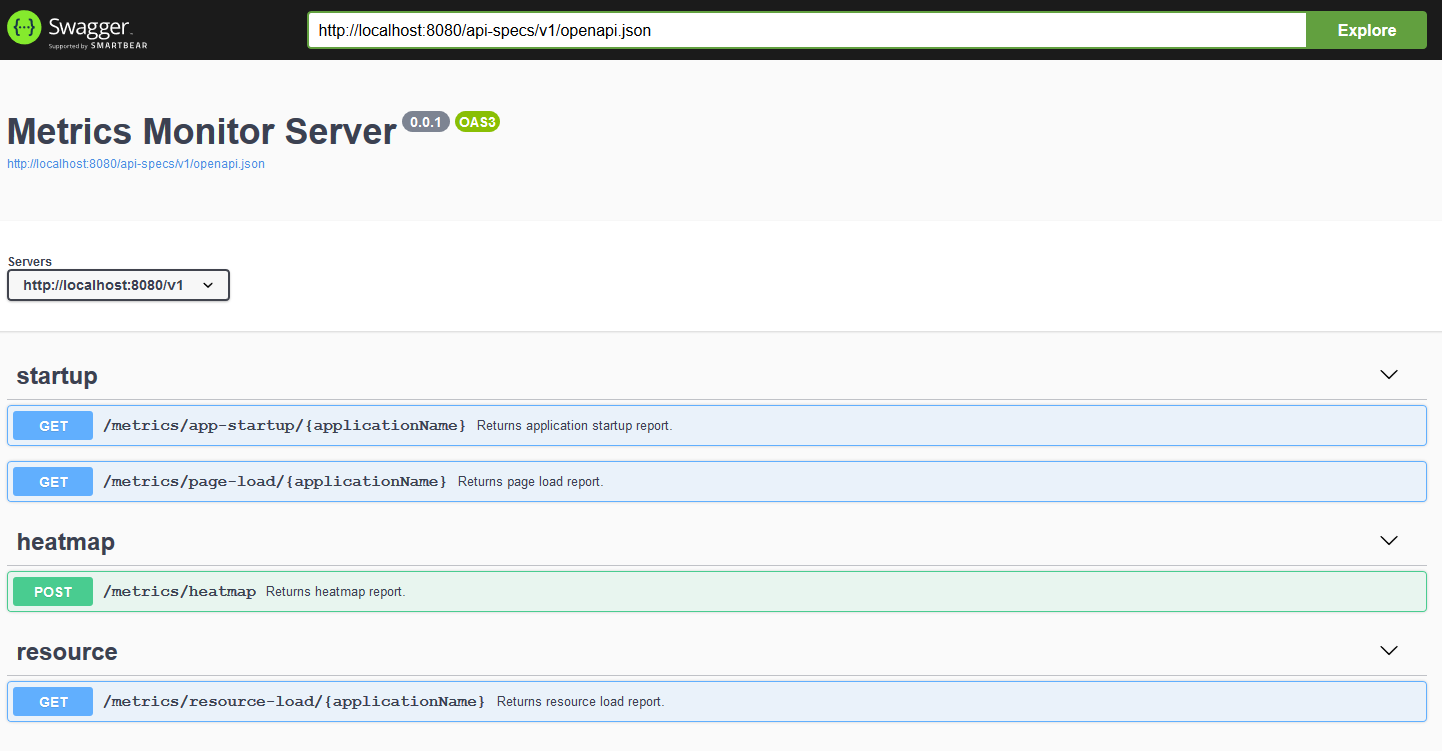
\includegraphics[width=0.9\textwidth]{swagger.png}
	\end{center}
	\caption{Swagger UI z izpostavljenimi dostopnimi točkami za pridobivanje poročil}
	\label{img:swagger}
\end{figure}

\subsection{Podporne tehnologije}
\label{ch3:sec2:sub3}

Za namestitev storitve za spremljanje metrik smo uporabili orodji za virtualizacijo Docker in Docker Compose. Storitev se zapakira v datoteko JAR, nato pa uporabimo to datoteko, da zgradimo sliko vsebnika Docker [Izvorna koda \ref{code:dockerfile}]. Ostali gradniki, od katerih je storitev odvisna -- Kafka, Zookeeper in podatkovna baza PostgreSQL, so ravno tako prenešeni v obliki slike Docker.

\begin{lstlisting}[label=code:dockerfile, caption=Dockerfile za storitev, float=h]
FROM openjdk:11-jre-slim

ENV JAVA_ENV=PRODUCTION
ENV KUMULUZEE_ENV_NAME=prod
ENV KUMULUZEE_ENV_PROD=true
ENV KUMULUZEE_DATASOURCES0_CONNECTIONURL=
  jdbc:postgresql://localhost:5432/metrics-monitor
ENV KUMULUZEE_DATASOURCES0_USERNAME=postgres
ENV KUMULUZEE_DATASOURCES0_PASSWORD=postgres
ENV KUMULUZEE_LOGS_LOGGERS0_LEVEL=INFO
RUN mkdir /app
WORKDIR /app
ADD ./api/target/metrics-monitor.jar /app
EXPOSE 8080
CMD ["java", "-jar", "metrics-monitor.jar"]
\end{lstlisting} 

Ker so gradniki tudi med seboj odvisni, moramo biti pozorni pri vrstnem redu zagona teh gradnikov. Proces lahko poenostavimo z uporabo orodja Docker Compose [Izvorna koda \ref{code:docker_compose}]. To orodje nam omogoča, da izpostavimo odvisnosti med gradniki katere zna nato pognati v pravilnem vrstnem redu. Zgrajene slike se hranijo v privatnem registru Docker, ki je gostovan na istem strežniku Nexus, kot prej omenjen repozitorij NPM.

\section{Prototip platforme za spremljanje metrik}
\label{ch3:sec3}

Ugotovitve prejšnjih poglavij smo uporabili tako, da smo razvili prototip platforme, ki metrike sprejema, shranjuje in prikazuje. V naslednjem delu bomo predstavili razviti izdelek in njegovo uporabo. Vsa koda, ki je bila razvita v procesu prototipiranja je objavljena na GitHubu in javno dostopna na naslovu \url{https://github.com/Jamsek-m/diploma-thesis}.

\subsection{Namestitev}
\label{ch3:sec3:sub1}

Namestitev te platforme sestoji iz dveh delov: namestitev zalednega dela, tj. storitve, ki metrike hrani in knjižnice, ki metrike zajema.

\subsubsection{Zaledni del}

Zaledni del ima veliko deležnikov, zaradi česar se priporoča uporaba orodja Docker Compose, saj nam namestitev zelo olajša. Vse kar potrebujemo je spisati docker-compose.yml datoteko, katere primer vidimo v izseku kode \ref{code:docker_compose}.

\begin{lstlisting}[label=code:docker_compose, caption=Primer datoteke docker-compose.yml]
version: "3"
networks:
 metrics-net:
   name: metrics-net
services:
  postgres:
    image: postgres
    ports:
      - "5433:5432"
    environment:
      POSTGRES_USER: postgres
      POSTGRES_PASSWORD: postgres
      POSTGRES_DB: metrics-monitor
    networks:
      - metrics-net
  zookeeper:
    image: wurstmeister/zookeeper
    ports:
      - "2181:2181"
    networks:
      - metrics-net
  kafka:
    image: wurstmeister/kafka
    ports:
      - "9092:9092"
    depends_on:
      - zookeeper
    environment:
      KAFKA_ADVERTISED_HOST_NAME: localhost
      KAFKA_ZOOKEEPER_CONNECT: zookeeper:2181
    networks:
      - metrics-net
  metrics-monitor-service:
    image: metrics-monitor-service
    ports:
      - "8080:8080"
    depends_on:
      - kafka
      - postgres
    environment:
      KUMULUZEE_DATASOURCES0_CONNECTIONURL:
          jdbc:postgresql://postgres:5433/metrics-monitor
      KUMULUZEE_DATASOURCES0_USERNAME: postgres
      KUMULUZEE_DATASOURCES0_PASSWORD: postgres
      KUMULUZEE_STREAMING_KAFKA_PRODUCER_BOOTSTRAPSERVERS:
          kafka:9092
      KUMULUZEE_STREAMING_KAFKA_CONSUMER_BOOTSTRAPSERVERS:
          kafka:9092
    networks:
      - metrics-net
\end{lstlisting}

Ko imamo tako datoteko spisano, se preprosto z ukazno lupino premaknemo v direktorij, kjer se ta datoteka nahaja in vpišemo ukaz \verb|docker-compose up|.

Docker Compose bo prebral to datoteko, prenesel vse potrebne slike vsebnikov, jih pognal v ustreznem vrstnem redu (ki smo ga v datoteki definirali z uporabo \verb|depends_on|) in povezal v skupno omrežje, da bodo lahko med seboj komunicirali.

\subsubsection{Namestitev in uporaba knjižnice}

Knjižnico za zajem metrik se v aplikacijo lahko vključi na dva načina. Prvi je klasični, kjer knjižnico naložimo kot datoteko Javascript z uporabo HTML elementa \verb|<script>|. Pri takem načinu uporabe je knjižnica dostopna preko globalnega objekta.

Drugi, priporočen način uporabe, je z namestitvijo knjižnice preko NPM-ja. To storimo s preprostim ukazom \verb|npm install --save metrics-monitor|. V takem primeru običajno uporabljamo kakšno orodje kot je Webpack, saj knjižnico vključimo samo v datoteko Javascript, to orodje pa nato zazna uporabo knjižnice in jo doda preostali kodi.

Naslednja demonstracija je vključitev knjižnice v aplikacijo, zgrajeno z ogrodjem Angular 8, katere koda je tudi dostopna na GitHubu.

\paragraph{Inicializacija aplikacije} 
Angular ob prvem zagonu kliče posebno metodo \verb|bootstrapModule()|, ki se nahaja v \verb|main.ts| [Izvorna koda \ref{code:lib_main_ts}].

\begin{lstlisting}[label=code:lib_main_ts, caption=Zagon Angular aplikacije]
if (environment.production) {
  enableProdMode();
}

platformBrowserDynamic().bootstrapModule(AppModule)
  .catch(err => console.error(err));
\end{lstlisting}

Tukaj moramo dodati inicializacijsko kodo za našo knjižnico. Metodi je treba dodati še nekaj parametrov in sicer URL naslov storitve, ki shranjuje metrike, način delovanja in ime aplikacije za razločevanje v primerih, ko spremljamo metrike več aplikacij. \\

\begin{lstlisting}[label=code:lib_main_ts_after, caption=Inicializacija knjižnice]
if (environment.production) {
  enableProdMode();
}

MetricsMonitor.init({
  applicationName: "angular-sample",
  mode: "capture",
  serverUrl: "http://localhost:8080",
  log: "debug",
  urlsWithParameters: [
    "/service/{id}"
  ]
}).then(() => {
  platformBrowserDynamic().bootstrapModule(AppModule)
    .catch(err => console.error(err));
}).catch((err: Error) => {
  console.error(err);
});
\end{lstlisting}

Kot je razvidno iz izvorne kode \ref{code:lib_main_ts_after}, imamo še dva opcijska parametra: prvi je stopnja beleženja dnevnika -- ko razvijamo in testiramo aplikacijo je bolje imeti sporočila z več podrobnostmi, ki jih v produkciji raje ne prikazujemo.

Drugi parameter pa pride prav, ko imamo dinamične strani. To so strani, ki spreminjajo vsebino glede na parameter URL, obdržijo pa enako strukturo. Na sliki \ref{img:heatmap}, kjer je prikazan vročinski zemljevid, vidimo seznam. Če kliknemo na katero izmed vrstic v seznamu, se nam odpre stran, ki prikazuje različne podatke glede na izbrano vrstico. Kar se spreminja je identifikacijski ključ elementa, ki določi katera vsebina se prikaže. Velikokrat je smiselno, da take strani združimo v eno, z uporabo ohranitvenika (ang. placeholder), kar nam uporaba tega parametra omogoča.

\paragraph{Zajem zagonskega časa aplikacije in začetka nalaganja pogleda}

To nastavimo v korenski komponenti (največkrat imenovani \verb|app.component.ts|), kot je to vidno v izvorni kodi \ref{code:lib_app_comp}.

\begin{lstlisting}[label=code:lib_app_comp, caption=Zajem zagonskega časa aplikacije in začetka nalaganja pogleda]
@Component({
  selector: "app-root",
  templateUrl: "./app.component.html",
  styleUrls: ["./app.component.scss"]
})
export class AppComponent implements OnInit {

  constructor(private router: Router) { }

  ngOnInit(): void {
    MetricsMonitor.logApplicationStartup();
    this.router.events.subscribe(routerEvent => {
      if (routerEvent instanceof NavigationStart) {
        MetricsMonitor.logPageLoadStart(routerEvent.url);
      }
    });
  }
}
\end{lstlisting}

Tukaj se poslužujemo znanja Aangularjevega življenskega cikla in modula Router.

Ko se angularjeva komponenta inicializira, preveri ali ta komponenta implementira metodo ngOnInit() in jo izvede. Ker je to korenska komponenta aplikacije, pomeni, da se je naša aplikacija uspešno zagnala, zato na tej točki zabeležimo končni zagonski čas aplikacije.

S poznavanjem modula Router (iz knjižnice \verb|@angular/router|) pa lahko zajamemo čas pričetka nalaganja pogleda. Tukaj namreč poslušamo za dogodke, ki jih Router proži. V Angularju je eden od teh dogodkov NavigationStart, ki se sproži, ko uporabnik zahteva spremembo pogleda.

\paragraph{Zajem časa nalaganja pogleda}

Ko se zabeleži čas nalaganja pogleda, se na strežnik pravzaprav ne pošlje še noben podatek. Da se zabeleži čas nalaganja strani in se podatki pošljejo na strežnik, moramo poklicati še metodo za beleženje konca nalaganja pogleda [Izvorna koda \ref{code:lib_page_comp}]. To postavimo na ustrezno mesto, ko je vsebina, pomembna za ta pogled naložena. Kaj je ustrezno mesto, pa zavisi od primera.

\begin{lstlisting}[label=code:lib_page_comp, caption=Zajem časa nalaganja pogleda]
@Component({
  selector: "app-first-page",
  templateUrl: "./first-page.component.html",
  styleUrls: ["./first-page.component.scss"]
})
export class FirstPageComponent implements OnInit, AfterViewInit {

  public displayedData: any[] = [];

  constructor(
      private router: Router,
      private dataService: DataService
  ) { }

  ngOnInit() {
    // 1. primerno mesto:
    // ko se komponenta za pogled instancira
    MetricsMonitor.logPageLoadEnd(this.router.url);
  }

  ngAfterViewInit(): void {
    // 2. primerno mesto:
    // ko se pogled izrise na zaslon
    MetricsMonitor.logPageLoadEnd(this.router.url);
  }

  private getData(): void {
    this.dataService.getData().subscribe(
      data => {
        this.displayedData = data;
        // 3. primerno mesto:
        // ko pridobimo podatke,
        // ki so bistveni za prikaz strani
        MetricsMonitor.logPageLoadEnd(this.router.url);
      }
    );
  }
}
\end{lstlisting}

\paragraph{Zajem premikov miške}

Knjižnica za zajem metrik ob inicializaciji registrira poslušalca dogodka premika miške. Ta poslušalec v ozadju beleži premike miške, jih shranjuje v medpomnilnik in, ko se ta napolni, posreduje strežniku. Razvijalcu tako za zajem te metrike ni potrebno storiti nič.

\section{Testiranje in poročila}
\label{ch3:sec4}

\subsubsection{Vročinski zemljevid}

Če hočemo iz vročinskega zemljevida kaj razbrati, moramo zemljevid projecirati na našo aplikacijo. To lahko storimo z zajemom zaslonskih mask na katere narišemo zemljevid, še boljši način pa je, da te podatke projeciramo kar v našo aplikacijo.

Knjižnica za zajem metrik ima dva načina delovanja. S prvim smo se že spoznali, ko smo zajemali metrike. Drugi način delovanja pa ne zbira metrik, ampak iz storitve za spremljanje metrik pridobi podatke o premikih miške, katere nato projeciramo.

Za delovanje projeciranja, moramo spremeniti našo kodo na dveh lokacijah. Prva je pri inicializaciji knjižnice [Izvorna koda \ref{code:heatmap_init}]. 

\begin{lstlisting}[label=code:heatmap_init, caption=Sprememba načina delovanja knjižnice]
MetricsMonitor.init({
  applicationName: "angular-sample",
  mode: "heatmap",
  serverUrl: "http://localhost:8080",
})
\end{lstlisting}

Ker pa ima vsaka stran svoj zemljevid, moramo še popraviti našo kodo tako, da se zemljevid na novo izriše, ko odpremo novo stran. To storimo s poslušanjem dogodkov Routerja, kot smo to počeli pri zbiranju časov nalaganja pogledov [Izvorna koda \ref{code:heatmap_redraw}].

\begin{lstlisting}[label=code:heatmap_redraw, caption=Sprememba zemljevida ob prehodu na novo stran]
this.router.events.subscribe(routerEvent => {
  if (routerEvent instanceof NavigationEnd) {
    MetricsMonitor.redrawHeatmap();
  } else if (routerEvent instanceof NavigationStart) {
    MetricsMonitor.logPageLoadStart(routerEvent.url);
  }	
});
\end{lstlisting}

Ko je to storjeno, odpremo aplikacijo v brskalniku, kjer se nam bo izrisal zemljevid, kot je viden na slikah \ref{img:heatmap1} in \ref{img:heatmap2}.

\begin{figure}[h]
	\begin{center}
		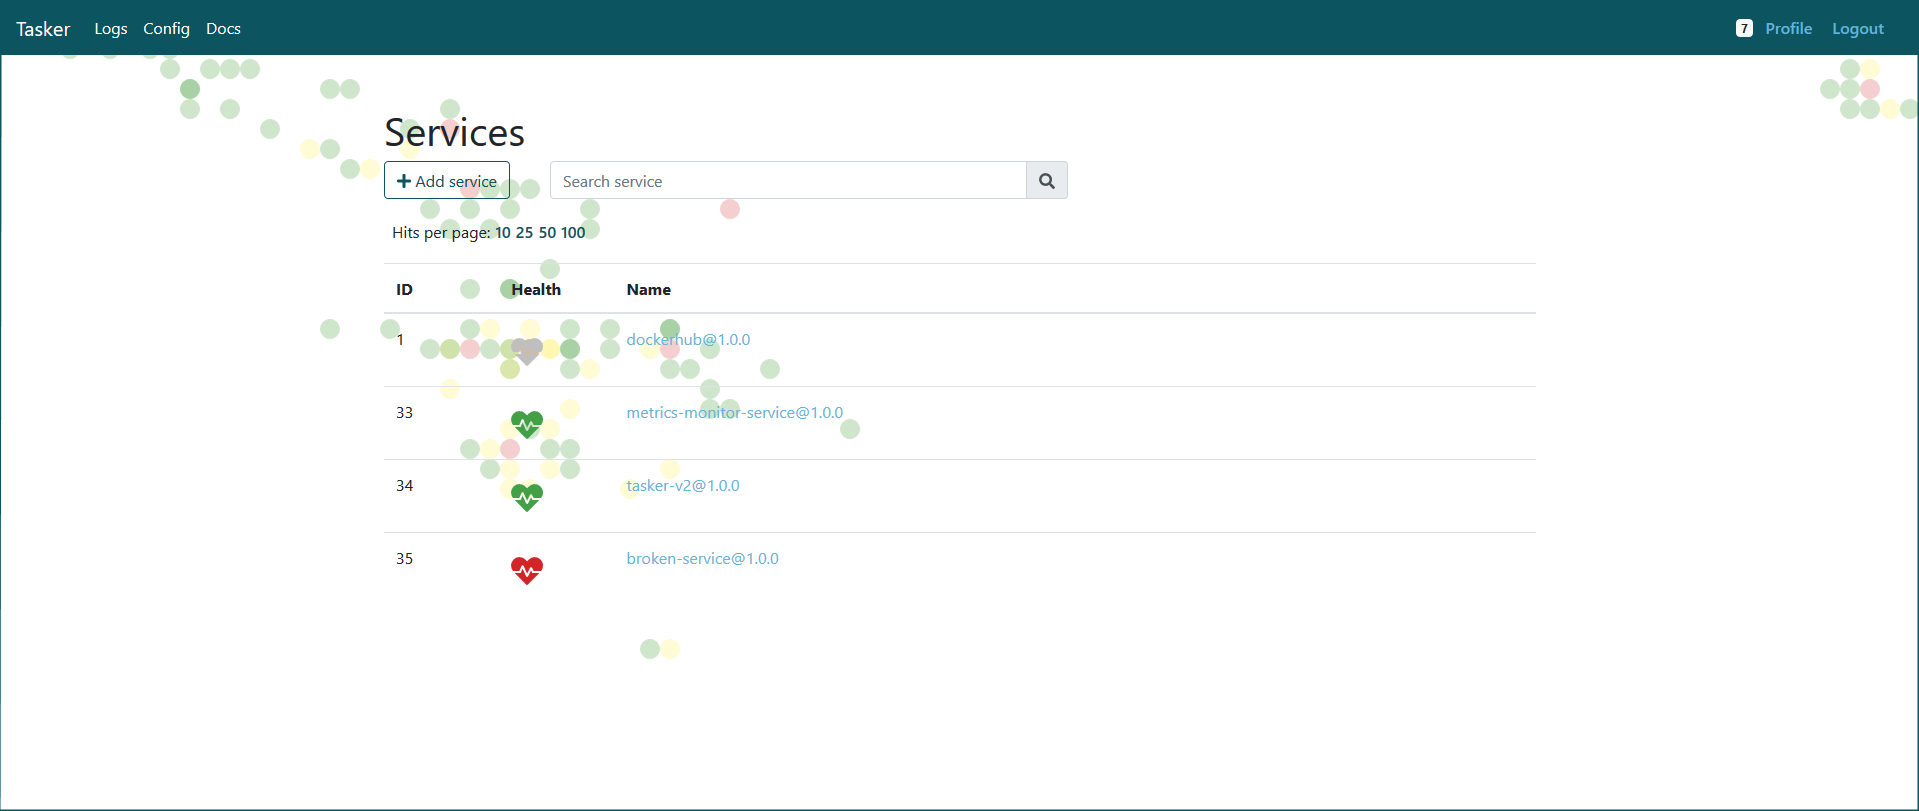
\includegraphics[width=1\textwidth]{heatmap_1.png}
	\end{center}
	\caption{Vročinski zemljevid za stran '/'}
	\label{img:heatmap1}
\end{figure}

\begin{figure}[h]
	\begin{center}
		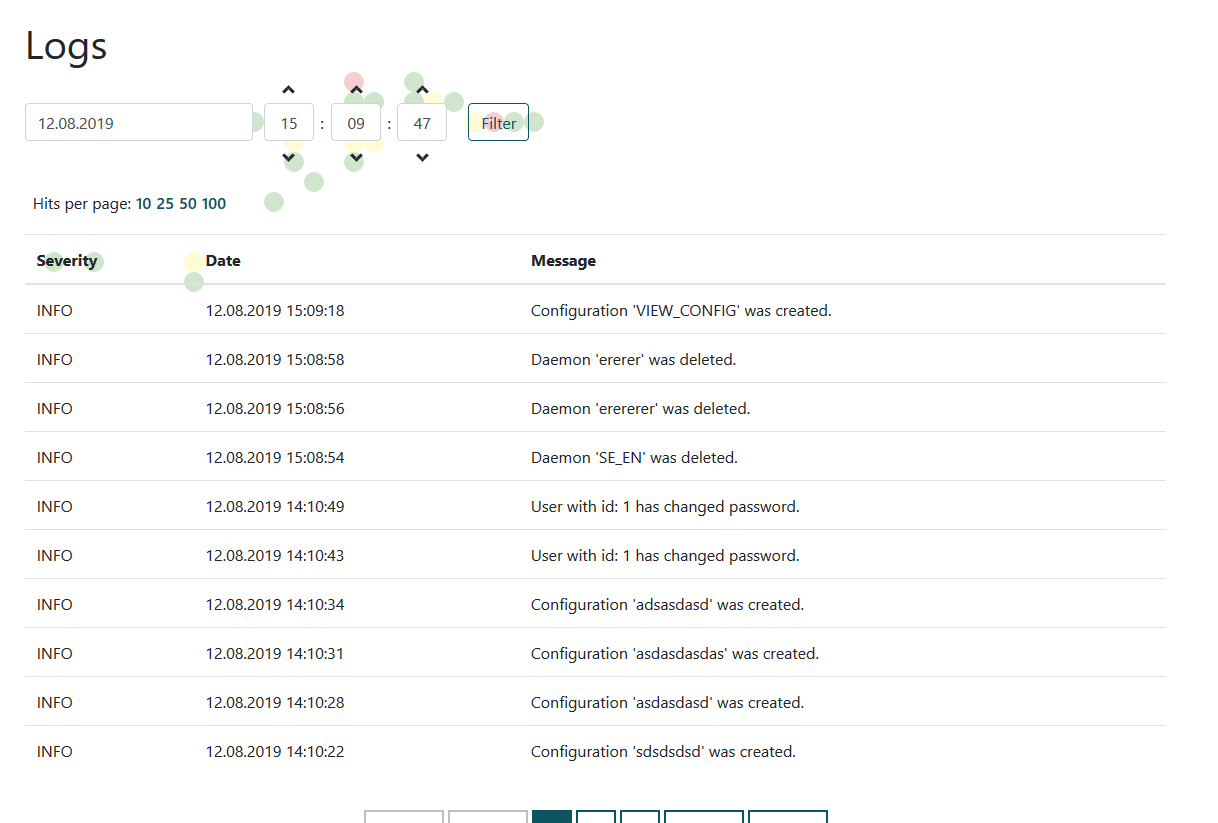
\includegraphics[width=1\textwidth]{heatmap_2.png}
	\end{center}
	\caption{Vročinski zemljevid  za stran '/logs'}
	\label{img:heatmap2}
\end{figure}

\subsubsection{Številske metrike}

Za ostale zajete metrike, ki so bolj formalne narave, imamo na voljo poročila (primeri vidni na  izvorni kodi \ref{code:app_startup_report}, \ref{code:page_load_report} in \ref{code:resource_load_report}).

Ta poročila lahko uporabimo za statistično analizo, s katero lahko ugotovimo, ali je naša aplikacija odzivna, ali se gradniki prenesejo iz strežnika dovolj hitro in če ne, na kolikšen del uporabnikov to vpliva.

\begin{figure}[h]
	\begin{center}
		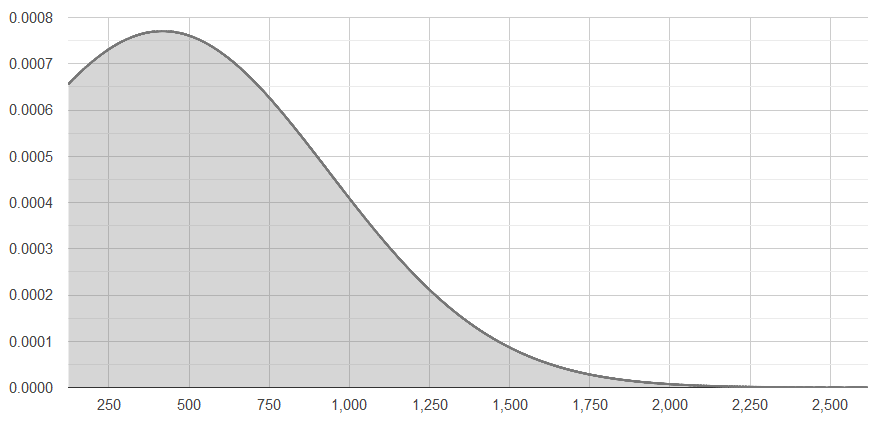
\includegraphics[width=1\textwidth]{app_startup_graph.png}
	\end{center}
	\caption{Zagonski časi aplikacije. Iz grafa se razbere, da se velikemu delu uporabnikov aplikacija zažene v približno 500ms, medtem, ko se majhnemu deležu uporabnikov aplikacija zažene v 1,5s ali več. Te številke potrdimo s pregledom poročila \ref{code:app_startup_report}.}
	\label{img:graph_app_startup}
\end{figure}

\begin{figure}[h]
	\begin{center}
		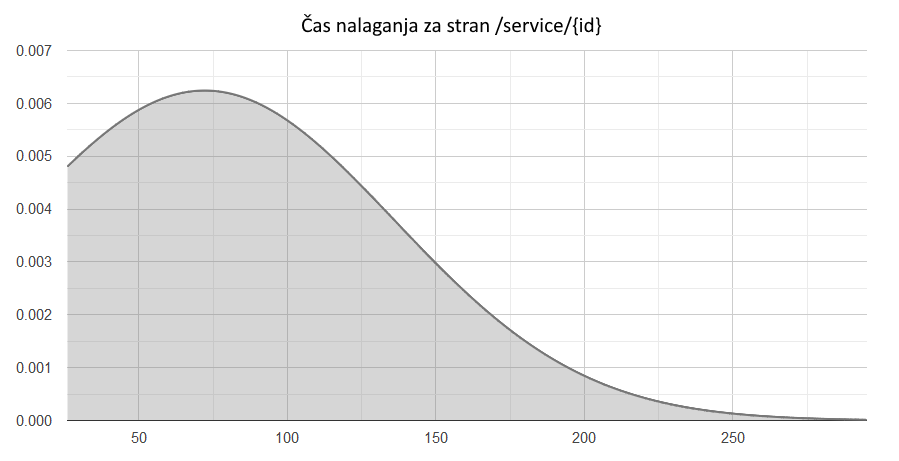
\includegraphics[width=1\textwidth]{page_load_graph_service_details.png}
	\end{center}
	\caption{Čas nalaganja pogleda '/service/:id'. Iz grafa se razbere, da se stran povečini naloži v 100ms, lahko pa tudi več, ampak ta čas ne presega 300ms, kar je precej dober čas.}
	\label{img:graph_page_load}
\end{figure}

Primeri grafov sicer uporabljajo podatke, ki so bili pridobljeni na precej majhni množici uporabnikov (n = 5). Pri tem sta dva uporabnika dostopala do aplikacije večkrat, saj so morale metrike zajeti tudi primere, ko so bile datoteke shranjene v predpomnilnik brskalnika. V realnem primeru je naša množica uporabnikov veliko večja, zaradi česar so tudi podatki bolj točni in tako lahko bolje ocenimo delovanje naše aplikacije.

Podatki, ponazorjeni s slikami \ref{img:heatmap1}, \ref{img:heatmap2}, \ref{img:graph_app_startup} in \ref{img:graph_page_load} so bili zajeti v lastni aplikaciji (razvojno ime Tasker), ki se razvija neodvisno od diplomskega dela. Za spremljanje metrik v tej aplikaciji smo se odločili zato, ker moramo za namestitev knjižnice za spremljanje metrik imeti poln dostop do izvorne kode aplikacije.

\section{Povzetek funkcionalnosti rešitve in evalvacija}

Razvita platforma nam omogoča spremljanje metrik zagonskega časa aplikacije, časa nalaganja pogleda, časa nalaganja gradnikov in spremljanja premikov miške. Te metrike spremljamo v realnem času in na aktualni bazi uporabnikov aplikacije. Zasnovana je tako, da ima minimalen vpliv na uporabnika aplikacije in na njegovo uporabniško izkušnjo. Platforma deluje neodvisno od uporabljenega ogrodja za razvoj enostranskih spletnih aplikacij, edini pogoj za uporabo je ta, da razvijalec dobro pozna delovanje uporabljenega ogrodja, da lahko umesti kodo za zajemanje metrik na ustrezno mesto.

Pri implementaciji zasnovane platforme smo odkrili tudi tehnične ovire pri spremljanju metrik. Osredotočili smo se na dve medsebojno povezani oviri -- veliko količino podatkov in dejstvo, da zbiranje metrik ne sme vplivati na uporabniško izkušnjo. Ti dve oviri smo obšli z uporabo praks za razvoj skalabilne programske opreme.

Pri zajemanju časa nalaganja gradnikov strani, smo opazili, da je velikost prenešenih gradnikov velikokrat enaka 0. To gre pripisati brskalnikovemu predpomnjenju teh gradnikov. Pri zajemanju te metrike, je tako smiselno izpustiti predpomnjene datoteke, saj se te niso prenašale in bi nam z ničelno vrednostjo pokvarile pravo sliko velikosti prenosa.

Razvita platforma dosega cilje, ki smo jih hoteli doseči. Razvijalcem omogoča spremljanje metrik v realnem času in to počne brez negativnega vpliva na uporabniško izkušnjo. Platforma spremlja metrike v katerikoli enostranski spletni aplikaciji, ne glede na uporabljeno ogrodje. S tem tudi poizkusimo standardizirati celoten proces spremljanja metrik in interpretacije rezultatov. Tega cilja ne dosegamo popolnoma. Da bi celoten proces bil res standardiziran, bi morali implementirati precej večje število spremljanih metrik. V nasprotnem primeru se mora razvijalec poslužiti še kakšne druge metode za zbiranje metrik, ki niso implementirane, s čimer otežimo standardizacijo.

\chapter{Sklepne ugotovitve}
\label{ch4}

Cilj diplomske naloge je bil zasnovati platformo za spremljanje metrik enostranskih spletnih aplikacij. Pri tem smo bili uspešni, saj nam je uspelo zasnovati in razviti platformo, ki metrike ustrezno spremlja in je neodvisna od uporabljenega ogrodja za gradnjo enostranskih spletnih aplikacij.

Z uporabo te platforme zagotavljamo, da se spremlja iste metrike, ne glede na uporabljene tehnologije. To nam omogoča lažjo namestitev in uporabo take platforme, pa tudi ne predstavlja dodatne ovire v primeru, da želimo zamenjati uporabljeno tehnologijo v naši aplikaciji, saj problemov s kompatibilnostjo ni. S prilagoditvijo metrik za enostranske spletne aplikacije pa smo dosegli, da so metrike bolj točne, kot na primer s prilagojeno uporabo orodja Google Analytics.

Za dosego tega, smo najprej raziskali kakšne metrike so sploh primerne za take aplikacije in v čem se razlikujejo od ostalih metrik. Iz teh metrik smo jih nato izbrali nekaj, ki so se nam zdele najbolj reprezentativne za enostranske aplikacije in najbolje demonstrirajo razliko v spremljanju metrik.

Člani W3C in razvijalci brskalnikov se pomena spremljanja metrik zavedajo, saj je v pripravi veliko osnutkov in predlogov za dodatne HTML5 API-je, ki izpostavljajo veliko uporabnih metrik. Večina teh predlogov, v času pisanja te naloge, žal, ni še nikjer blizu implementacije. Najdemo jih tako v opuščanju, ali pa le v določenih brskalnikih (kot eksperimentalne funkcionalnosti). Ko bodo tej API-ji standardizirani in implementirani, bomo lahko dobili izredno natančno in celovito predstavo obnašanja naše aplikacije.

Za nadaljnje delo na zasnovani platformi, pa ni potrebno čakati na implementacijo novih API-jev. Veliko metrik, opisanih v poglavju \ref{ch1:sec5}, se ne zanaša na te nove API-je in lahko njihovo spremljanje precej hitro implementiramo. Smiselno je dodati tudi grafični vmesnik, ki nam te podatke prikaže v neki človeku bolj prijazni obliki. S tem lahko metrike približamo tudi nekomu, ki nima tehničnega znanja.

Da zaključimo, dela je še veliko in ga razvijalcem, z interesom zbiranja metrik, ne bo zmanjkalo.

\newpage %dodaj po potrebi, da bo številka strani za Literaturo v Kazalu pravilna!
\ \\
\clearpage
\addcontentsline{toc}{chapter}{Literatura}
\bibliographystyle{plain}
\bibliography{literatura}


\end{document}

